\chapter{\textgreek{Πειράματα και Αποτελέσματα}}
\label{chapter_5}
\pagestyle{fancy}
\fancyhf{}
%\fancyhead[OC]{\leftmark}
%\fancyhead[C]{}
%\fancyhead[EC]{\rightmark}
\renewcommand{\footrulewidth}{0.5pt}
\cfoot{\thepage}

\section{\textgreek{Εκπαίδευση των Νευρωνικών Δικτύων}}
\textgreek{Σε αυτο το κομμάτι θα παρουσιάσουμε μερικές τεχνικές τις οποίες εφαρμόσαμε για την εκπαίδευση των ΠΣΝΔ καθώς και κάποιες υπερ-παραμέτρους που θέσαμε κατά την διαδικασία της εκπαίδευσης. Η εκπαίδευση των ΠΣΝΔ αποτελεί μια χρονοβόρα διαδικασία και επειδή μπορεί να πάρει μέρες για να συγκλίνει, κρίναμε απαραίτητη την τοποθέτηση κάποιων σημείων ελέγχου κατά την διαδικασία της εκπαίδευσης. }

\subsection{\textgreek{Σημεία Ελέγχου} (Checkpoints)}
\textgreek{Τα σημεία ελέγχου αποτελούν ένα απαραίτητο κομμάτι για την διαδικασία της εκπαίδευσης, ειδικά όταν έχουμε ΠΣΝΔ βαθειάς μάθησης. Η διαδικασία της μάθησης μπορεί να πάρει πολύ χρόνο, όπως στην δική μας περίπτωση που ήταν μερικές μέρες μέχρι να φτάσουμε σε σύγκλιση. Επομένως, πρέπει να αποθηκεύουμε τις παραμέτρους που μαθαίνει το ΠΣΝΔ κατά την μάθηση για να μην συμβεί κάποια αστοχία και χρειαστεί να κάνουμε την διαδικασία της μάθησης από την αρχή.
\par
Για το δικό μας μοντέλο θέσαμε ως σημείο ελέγχου το τέλος της κάθε εποχής} (epoch),\textgreek{ όπου αποθηκεύουμε τις παραμέτρους μας σε περίπτωση που χρειαστεί να συνεχίσουμε την εκπαίδευση του ΠΣΝΔ από εκείνο το σημείο. Ο όρος 'Εποχή' αντιπροσωπεύει την τροφοδοσία ενός ΝΔ με το σύνολο δεδομένων εκπαίδευσης. Η διαδικασία η οποία ολόκληρο το σύνολο δεδομένων εκπαίδευσης περνά μία φορά από το στάδιο της εμπρόσθιας διάδοσης και της οπισθοδρόμησης αντίστοιχα ορίζεται ως 'Εποχή'.  Ιδανικά, στο τέλος κάθε εποχής ελέγχουμε τα αποτελέσματα της μάθησης, επομένως αν υπάρχει κάποια βελτίωση στην διαδικασία της μάθησης, ελέγχοντας την ακρίβεια του μοντέλου στο σύνολο δεδομένων επαλήθευσης που χρησιμοποιούμε }(validation set) \textgreek{στο τέλος κάθε εποχής τότε αποθηκεύουμε τα βάρη του. }

\subsection{\textgreek{Πρώιμο Σταμάτημα} (Early Stopping)}
\textgreek{Το πρώιμο σταμάτημα είναι ένας μηχανισμός ο οποίος αποσκοπεί στην αποδοτικότητα της εκπαίδευσης του ΠΣΝΔ. Αποσκοπεί στην αποτροπή του μοντέλου από την κατάσταση της υπερ-μάθησης }(over-fitting). \textgreek{Ελέγχουμε το σφάλμα από το σύνολο επαλήθευσης σε κάθε εποχή, αν δεν υπάρχει κάποια μείωση του σφάλματος για 12 συνεχόμενες εποχές, τότε σταματάει η διαδικασία της μάθησης. Με αυτόν τον τρόπο σταματάει η διαδικασία της μάθησης πριν το μοντέλο αρχίσει να μαθαίνει υπερβολικά το σύνολο δεδομένων της εκπαίδευσης το οποίο αποτελεί πρόβλημα.}

\subsection{\textgreek{Ρυθμός Μάθησης}}
\textgreek{Ο ρυθμός μάθησης είναι από τις πιο σημαντικές παραμέτρους για την εκπαίδευση των ΝΝ. Χρειάζεται να είναι μικρό το μέγεθος για να συγκλίνει, αλλά όχι πολύ μικρό ώστε να πάρει πάρα πολύ χρόνο να βρεθεί σε σύγκλιση. Για την εκπαίδευση των ΣΝΔ βρήκαμε την βέλτιστη τιμή του ρυθμού μάθησης να είναι $10^{-3}$ χρησιμοποιώντας τον αλγόριθμο} Adam \textgreek{ ως αλγόριθμο βελτιστοποίησης. Ενώ για την εκπαίδευση του ΣΝΔ μαζί με το ΤΥΣΠ-ΕΝΔ βρήκαμε σαν βέλτιστη επιλογή την χρήση ενός πολύ μικρότερου ρυθμού μάθησης το οποίο ήταν $10^{-13}$ σε συνδυασμό με τον αλγόριθμο βελτιστοποίησης} SGD \textgreek{και με χρήση της παραμέτρου της ορμής επιλεγμένη στο 0.9. Για την ακρίβεια, ξεκινήσαμε με ρυθμό μάθησης $10^{-6}$ και σταδιακά δοκιμάστηκαν και μικρότεροι ρυθμοί μάθησης μέχρι να καταλήξουμε στο $10^{-13}$. }



\section{\textgreek{Αποτελέσματα}}
\textgreek{Τα μοντέλα εκπαιδεύτηκαν σε 2975 εικόνες μεγέθους $512\times 512$ η κάθε μία, ενώ το σύνολο των εικόνων επαλήθευσης το οποίο χρησιμοποιούμε για την επαλήθευση του μοντέλου στο τέλος της κάθε εποχής είναι 500 εικόνες. Επίσης οι εικόνες έχουν επαληθευτεί στο κανονικό τους μέγεθος ($1024\times 2048$). Τα μοντέλα εκπαιδεύτηκαν σε παρτίδες }(batches) \textgreek{όπου το μέγεθος ήταν 2 και 4 εκτός από την ολοκληρωμένη εκπαίδευση του }end-to-end \textgreek{μοντέλου ΠΣΝΔ-ΤΥΣΠ-ΕΝΔ που χρησιμοποιήθηκε μέγεθος ίσο με ένα λόγω των περιορισμένων διαθέσιμων πόρων. Τα αποτελέσματα στον πίνακα }\ref{table:results_table_1} \textgreek{μας δείχνουν τις επιδόσεις των ΠΣΝΔ σε συνδυασμό με την μονάδα επεξεργασίας Μέσου Φίλτρου καθώς δοκιμάζουμε τις επιδόσεις με διαφορετικό μέγεθος παραθύρου, ενώ ο πίνακας }\ref{table:results_table_2} \textgreek{επιδεικνύει τις επιδόσεις του μοντέλου με μονάδα μετα-επεξεργασίας ΤΥΣΠ-ΕΝΔ καθώς και την σύγκριση με τις αναδρομικές επαναλήψεις κατά την δοκιμή. Η δοκιμή του μοντέλου έγινε στα δεδομένα επαλήθευσης, δηλαδή στις 500 εικόνες.} 


\textgreek{Η μετρική που χρησιμοποιούμε στα αποτελέσματα είναι ένας μέσος όρος του πλήθους των επιτυχών προβλέψεων του μοντέλου ως προς το άθροισμα των λανθασμένων προβλέψεων του μοντέλου μαζί με τα $TP$ για την κάθε εικόνα. Πιο συγκεκριμένα μετράμε συνολικά από όλη την εικόνα τις παραμέτρους }$TP, FP, FN$ \textgreek{και υπολογίζουμε την συνάρτηση $J$. Επομένως μετράμε την συνάρτηση }Jaccard Similarity ($J$) \textgreek{(εξίσωση }\ref{eqn:jaccard}) \textgreek{ή} Intersection over Union \textgreek{από κάθε εικόνα και παίρνουμε έναν μέσο όρο από τις 500 εικόνες που χρησιμοποιήσαμε για την δοκιμή του μοντέλου (εξίσωση} \ref{eqn:mean_jaccard}). \textgreek{Επίσης, κατά την μέτρηση του μοντέλου δεν λάβαμε υπόψη μας τα εικονοστοιχεία τα οποία είναι ταξινομημένα ως 'Κενά'. Δηλαδή, αν ένα εικονοστοιχείο έχει ταξινομηθεί σε μία οποιαδήποτε κλάση $i$ και ανήκει στην κλάση 'Κενό' τότε δεν συνεισφέρει στο αποτέλεσμα.}

\noindent\begin{minipage}{.5\linewidth}
  \begin{equation}
  \label{eqn:jaccard}
    \begin{split}
  J &= \frac{TP}{TP+FP+FN}\\[1cm]
  TP &= \texttt{True Positives}\\ 
  FP &= \texttt{False Positives}\\
  FN &= \texttt{False Negatives}\\
  \end{split}
  \end{equation}
\end{minipage}%
\begin{minipage}{.5\linewidth}
  \begin{equation}
  \label{eqn:mean_jaccard}
  mIoU = \frac{1}{N}\sum_{i=1}^{N} J(i)
  \end{equation}
\end{minipage}
  
%%%%%%% ΕΔΩ ΚΑΤΩ Ο ΚΑΚΟΣ ΧΑΜΟΣΣΣΣΣΣΣ %%%%%%%%%%%%%%%%%%%%%%%%%%%%%%
True Positives \textgreek{συμβολίζονται τα εικονοστοιχεία τα οποία έχουν προβλεφθεί σωστά από τον ταξινομητή. Από την σκοπιά της στατιστικής, } False Positives \textgreek{είναι όταν το μοντέλο που έχει προβλέψει ένα αποτέλεσμα απορρίπτει την αναγνώριση του σωστού αποτελέσματος λανθασμένα. Ενώ }False Negatives \textgreek{είναι όταν το μοντέλο λανθασμένα απέτυχε να απορρίψει το αποτέλεσμα που πρόβλεψε.} 
\par 
%%%%%%%%%%%%%%%%%%%%%%%%%%%%%%%%


  

\begin{table}[H]
 \begin{adjustwidth}{-0.8cm}{}
\scalebox{0.8}{
\begin{tabular}{l|llllllllll}
\hline
\textbf{Model}     & - & 9x9  & 19x19    & 31x31 & 45x45 & 59x59 & 65x65 & 71x71 & 77x77 & 81x81 \\ \hline
SD-CNN-MFB & 0.607106 & 0.60792& 0.60847& 0.60905& 0.60960 & 0.60997 & \textbf{0.60998}& 0.60989& 0.60976& 0.60957\\ 
SD-CNN     &0.76681 & 0.76711& \textbf{0.76716}  & 0.76684& 0.76574& 0.76380& 0.76265& 0.76136 & 0.75996& 0.75897\\%\hline
SD-CNN-CRF[3] & 0.62051 & 0.62132& 0.62186& 0.62251& 0.62316& 0.62352& \textbf{0.62355} & 0.62345& 0.62322& 0.62303\\
BD-CNN     & 0.80342 & 0.80360 & \textbf{0.80373}& 0.80351  & 0.80234& 0.80001 & 0.79857& 0.79695& 0.79509 & 0.79375 \\

\end{tabular}
}
\caption[\textgreek{Αποτελέσματα Μέσου Φίλτρου}]{\textgreek{Αποτελέσματα των ΠΣΝΔ με τον αλγόριθμο Μέσου Φίλτρου ως μονάδα μετα-επεξεργασίας χρησιμοποιώντας διαφορετικά μεγέθη παραθύρων.} SD (Strided Deconvolution) \textgreek{είναι η μονάδα με αποκωδικοποίησης με βήμα ολίσθησης ενώ }BD (Bilinear Deconvolution) \textgreek{είναι η διγραμμική μονάδα αποκωδικοποίησης. Με }MFB (Median Frequency Balance) \textgreek{συμβολίζουμε την συνάρτηση ισοστάθμισης που χρησιμοποιήσαμε.}}\label{table:results_table_1}
\end{adjustwidth}
\end{table}

\textgreek{Όπως φαίνεται στον πίνακα }\ref{table:results_table_1} \textgreek{το μεσαίο φίλτρο δεν προσδίδει ιδιαίτερη βελτίωση στα αποτελέσματα παρά μόνο μια μικρή εξομάλυνση. Για την ακρίβεια η βελτίωση είναι της τάξης του $0.2\%$. }
\par
\textgreek{Τα μοντέλο }SD-CNN \textgreek{το οποίο εκπαιδεύτηκε με την συνάρτηση ισοστάθμισης μέσης συχνότητας πήρε 70 εποχές μέχρι να επιτευχθεί σύγκλιση καθώς επειδή προσπαθεί το ΣΝΔ να μάθει πληροφορία από όλες τις κλάσεις ανεξάρτητα της δυσαναλογίας χρειάζεται περισσότερο χρόνο για την σύγκλιση εφόσον η λανθασμένη ταξινόμηση ενός εικονοστοιχείου που βρίσκεται σε μια σπάνια κατηγορία διαδίδει μεγαλύτερο σφάλμα προς τα πίσω στο ΣΝΔ. Τα ΣΝΔ που εκπαιδεύτηκαν χωρίς ισοστάθμιση, χρειάστηκαν μόνο 40 εποχές για να συγκλίνουν καθώς βρέθηκαν πολύ γρήγορα σε κατάσταση υπερμάθησης.}
\par

\textgreek{Ο πίνακας} \ref{table:results_table_2} \textgreek{δείχνει την επίδοση του μοντέλου }SD-CNN \textgreek{μαζί με την μονάδα μετα-επεξεργασίας ΤΥΣΠ-ΕΝΔ} (CRF-RNN). \textgreek{Αρχικά επιχειρήσαμε να παγώσουμε την μάθηση στο ΠΣΝΔ και να γίνει η εκπαίδευση μόνο στο ΤΥΣΠ-ΕΝΔ όμως δεν υπήρχε κάποιο θετικό αποτέλεσμα. Εν τέλει, ξεκινήσαμε να εκπαιδεύσουμε το ΠΣΝΔ σε συνδυασμό με το ΤΥΣΠ-ΕΝΔ αρχικά με 10 επαναλήψεις και με ρυθμό μάθησης $10^{-6}$ για να δούμε την ανταπόκριση του μοντέλου. Σταδιακά μειώσαμε τον ρυθμό μάθησης σε $10^{-13}$ όμως ακόμα και μετα από 20 εποχές το μοντέλο άρχισε να αποκλίνει. Πιθανότητα λόγω των πολλών επαναλήψεων στο ΤΥΣΠ-ΕΝΔ παρουσιάστηκε το φαινόμενο της εξαφάνισης των αποκλίσεων. Επομένως μειώσαμε τον αριθμό των επαναλήψεων σε 5 κατά την μάθηση και πετύχαμε σύγκλιση μετα από 30 εποχές.
\par 
Το πρόβλημα με τους γράφους είναι ότι στηρίζονται πάρα πολύ στον ταξινομητή (ΣΝΔ) που τα τροφοδοτεί για να συνεισφέρουν περισσότερο στην επίδοση. Στην προκειμένη περίπτωση πετύχαμε μια βελτίωση της τάξης του 1\%. Από τον πίνακα }\ref{table:results_table_2} \textgreek{είναι ολοφάνερο πως όσο αυξάνονται οι επαναλήψεις επιβαρύνεται με επιπλέον χρόνο το μοντέλο καθώς σε κάθε επανάληψη γίνεται επανεκτίμηση της κατανομής. Για περισσότερες από 3 επαναλήψεις το μοντέλο δεν παρουσιάζει κάποια βελτίωση, επίσης στον πίνακα βλέπουμε και τον χρόνο της συμπερασματολογίας καθώς και μια τυπική απόκλιση του χρόνου σε δευτερόλεπτα που μετρήσαμε από την συμπερασματολογία 500 εικόνων.}

\begin{table}[H]
\centering
\begin{tabular}{lccc}
\hline
\textbf{Model[Iterations]}  & \textbf{mean IoU} & \textbf{\textgreek{Χρόνος  Διεκπεραίωσης}[s]} & \textbf{\textgreek{Απόκλιση Χρόνου}} \\ \hline
SD-CNN      & 0.60710            & 0.1111              & 0.06               \\ %\hline
SD-CNN-CRF{[}3{]}  & 0.62058              & 0.3988              & 0.09               \\ %\hline
SD-CNN-CRF{[}5{]}  & 0.62051            & 0.6994              & 0.17               \\ %\hline
SD-CNN-CRF{[}10{]} & 0.62051            & 1.1868              & 0.09               \\ %\hline
SD-CNN-CRF{[}20{]} & 0.62051 & 2.5681 & 0.48 \\

\end{tabular}

\caption[\textgreek{Αποτελέσματα} CNN-CRF]{\textgreek{Σύγκριση των μοντέλων με την μονάδα μετα-επεξεργασίας ΤΥΣΠ-ΕΝΔ με διαφορετικό αριθμό επαναλήψεων.}}\label{table:results_table_2}
\end{table}


\textgreek{Στον πίνακα }\ref{table:results_table_3} \textgreek{βλέπουμε την ακρίβεια του μοντέλου μας σε σχέση με τα σύγχρονα μοντέλα στο }test set \textgreek{του συνόλου δεδομένων. Για τα αποτελέσματα χρησιμοποιήθηκε η μετρική }IoU \textgreek{της εξίσωσης }\ref{eqn:jaccard} \textgreek{με την διαφορά ότι υπολογίστηκε για κάθε κλάση και ο μέσος όρος βγήκε από τον αριθμό των κλάσεων που υπάρχουν σε κάθε εικόνα. Στην δεξιά στήλη βλέπουμε την ακρίβεια που είχαν τα μοντέλα στην σωστή ταξινόμηση των εικονοστοιχείων σε μια από της εφτά υπερ-κατηγορίες. Το σύνολο δεδομένων αποτελείται από $1525$ εικόνες, ενώ η αξιολόγηση έγινε στον }server \textgreek{της βάσης }Cityscapes \cite{Cityscapes}. \textgreek{Ο πίνακας }\ref{table:results_table_4} \textgreek{μας δείχνει την ακρίβεια των μοντέλων για την αναγνώριση της κάθε κατηγορίας.}

\begin{table}[H]
\centering
\begin{tabular}{lccc}
\hline
\textbf{Model}  & \textbf{mean IoU Class} & \textbf{mean IoU Category}\\ \hline
PSPNet \cite{pspnet}  & 80.2     & 90.2   \\ %\hline
ResNet-DUC-HDC \cite{duc_hdc} & 80.1 & -\\
GRN-LRN-ResNet \cite{DBLP:conf/ijcai/ZhangTLLY17} & 77.27& - \\
PEARL-ResNet101 \cite{video_scene_parsing}& 74.9 & -\\ %\hline
RefineNet-ResNet101 \cite{RefineNet}& 73.06    & -         \\ %\hline
AdapNet \cite{adapNet}& 72.91 & -\\
SD-CNN-CRF{[}3{]} (Ours)  & 34.08  &  60.15  \\ %\hline
\end{tabular}

\caption[\textgreek{Σύγκριση με σύγχρονα μοντέλα}]{\textgreek{Σύγκριση του μοντέλου μας με σύγχρονα μοντέλα στο }test set.}\label{table:results_table_3}
\end{table}

\textgreek{Τα περισσότερα μοντέλα που κατέχουν τις πρώτες θέσεις διαθέτουν πολύ βαθιά ΣΝΔ με εκατοντάδες εκατομμύρια παραμέτρους εν αντιθέσει με το δικό μας μοντέλο το οποίο διαθέτει μόλις $7$ εκατομμύρια. Το }PSPNet \textgreek{για παράδειγμα διαθέτει ένα προ-εκπαιδευμένο ΣΝΔ }(ResNet) \textgreek{με $101$ επίπεδα συνέλιξης το οποίο είχε εκπαιδευτεί πρώτα σε ένα άλλο σύνολο δεδομένων }(ImageNet) \textgreek{και αποσκοπούσε στην εξαγωγή πολύπλοκων χαρακτηριστικών για την τροφοδοσία του ΣΝΔ }(PSPNet) \textgreek{ το οποίο πέτυχε την πρώτη θέση στην κατάταξη.}

\begin{table}[H]
  \begin{adjustwidth}{-1.5cm}{}
  \scalebox{0.55}{
    \begin{tabular}{l|ccccccccccccccccccc}
      \hline
      \textbf{Model}  & road & sidewalk & building& wall &fence & pole &traffic light&traffic sign & vegetation &terrain &sky & person &rider &car & truck &bus & train & motorcycle & bicycle \\ \hline
SD-CNN-CRF{[}3{]} & 86.99  &  44.03 & 60.00 & 14.35 & 9.20 & 9.60 & 10.86 & 10.54 & 70.72 & 49.31 & 81.04 &27.55& 18.26 &71.99&10.51&18.33&21.49&7.13 &25.64  \\ %\hline
    \end{tabular}}
    \caption[\textgreek{Αποτέλεσμα μοντέλου ανά κατηγορία}]{\textgreek{Αποτελέσματα για κάθε κατηγορία από τον }server \textgreek{της βάσης με την μετρική} IoU (\%).}\label{table:results_table_4}
  \end{adjustwidth}
\end{table}

\textgreek{Όπως μπορούμε να δούμε από τον πίνακα }\ref{table:results_table_5} \textgreek{βλέπουμε ότι τα αποτελέσματα σε επίπεδο υπερ-κατηγορίας είναι αρκετά ανεβασμένα. Αυτό μας δείχνει ότι το μοντέλο μπερδεύει περισσότερο τα εικονοστοιχεία τα οποία βρίσκονται στην ίδια υπερ-κατηγορία. Αντιθέτως, τα αποτελέσματα για τις υπερ-κατηγορίες 'Αντικείμενο' }(object) \textgreek{και 'Άνθρωπος'} (human) \textgreek{είναι αρκετά χαμηλά. Μια εξήγηση σε αυτό είναι η αναλογία των εικονοστοιχείων που ανήκουν σε αυτές τις υπερ-κατηγορίες σε σχέση με τα υπόλοιπα εικονοστοιχεία. Τα εικονοστοιχεία που ανήκουν στις παραπάνω υπερ-κατηγορίες είναι πολύ λιγότερα σε σχέση με τα υπόλοιπα και αυτή η μεγάλη δυσαναλογία δεν μπορεί να αντιμετωπιστεί εύκολα από την μέθοδο ισοστάθμισης κλάσεων. Επίσης τα αντικείμενα που ανήκουν σε αυτές τις κατηγορίες είναι πιο δύσκολο να αναγνωριστούν στην εικόνα.}

\begin{table}[H]
 \begin{tabular}{l|ccccccc}
  \hline
  \textbf{Model} & flat & nature & object & sky & construction & human & vehicle \\ \hline
    SD-CNN-CRF{[}3{]} & 93.42 & 71.01 & 14.67 & 81.04 & 60.19 & 30.60 & 70.15
 \end{tabular}
  \caption[\textgreek{Αποτέλεσμα ανά υπερ-κατηγορία}]{\textgreek{Αποτελέσματα μοντέλου ανά υπερ-κατηγορία στο }test set.}\label{table:results_table_5}
\end{table}


\textgreek{Παρακάτω βλέπουμε μερικές εκτιμήσεις πάνω σε εικόνες από τα μοντέλα που παρουσιάσαμε. Στην εικόνα }\ref{fig:image_results_1} \textgreek{βλέπουμε τα αποτελέσματα από μια εικόνα εισόδου στο μοντέλο }SD-CNN-CRF \textgreek{το οποίο έχει εκπαιδευτεί με ισοστάθμιση κλάσεων. Σε γενικές γραμμές έχει καταφέρει να τμηματοποιήσει αρκετά από τα αντικείμενα αν και όχι στη πιο λεπτομερή μορφή. Ο λόγος πιθανότητα που υπάρχει μια αστοχία και μια υπερκατάτμηση σε αντικείμενα όπως οι πινακίδες κυκλοφορίας και τα φανάρια κυκλοφορίας είναι η συμπίεση που υπέστη το μοντέλο από τα τμήματα συγκέντρωσης τα οποία χάνουν αρκετή πληροφορία ενώ τα επίπεδα υπερδειγματοληψίας φαίνεται να μην μπορούν να ανταπεξέλθουν σε αυτό το πρόβλημα. Επίσης, το μεσαίο φίλτρο ομαλοποιεί κάπως κάποια απομακρυσμένα εικονοστοιχεία από την κατηγορία τους τα οποία έχουν ταξινομηθεί σε λάθος κατηγορία.} 
\newpage
\textgreek{Στην εικόνα }\ref{fig:image_results_2} \textgreek{βλέπουμε το ίδιο μοντέλο ΠΣΝΔ με προηγουμένως χωρίς να έχει εκπαιδευτεί με κάποια συνάρτηση ισοστάθμισης. Αυτό είναι προφανές καθώς το ΠΣΝΔ έχει μάθει πολύ λιγότερες κατηγορίες, δηλαδή τις επικρατέστερες κατά πλειοψηφία. Αν και το ΠΣΝΔ έχει μάθει αρκετά καλά τις επικρατέστερες κλάσεις, γενικά αδυνατεί να αναγνωρίσει οποιαδήποτε άλλη κλάση.}\par

\textgreek{Τέλος, στην εικόνα }\ref{fig:image_results_3} \textgreek{βλέπουμε ένα δείγμα από το μοντέλο με την διγραμμική αποκωδικοποίηση το οποίο δεν έχει εκπαίδευση με την συνάρτηση για την δυσαναλογία των κλάσεων. Κάτι που παρατηρούμε είναι πως αν και χωρίς ισοστάθμιση κλάσεων καταφέρνει να αναγνωρίσει περισσότερα εικονοστοιχεία στην εικόνα εισόδου που ανήκουν και σε κλάσεις που αποτελούν μειονότητα. Μια εξήγηση για αυτό είναι ότι το προηγούμενο μοντέλο διαθέτει περισσότερες παραμέτρους λόγω του τμήματος υπερδειγματοληψίας που διαθέτει με εκπαιδευόμενες παραμέτρους τείνει να πάσχει από μεγαλύτερο πρόβλημα υπερμάθησης.}


%%%% IMAGE PREDICTIONS
\begin{figure}[H]
 \centering
 \begin{subfigure}[b]{\linewidth}
  \centering
  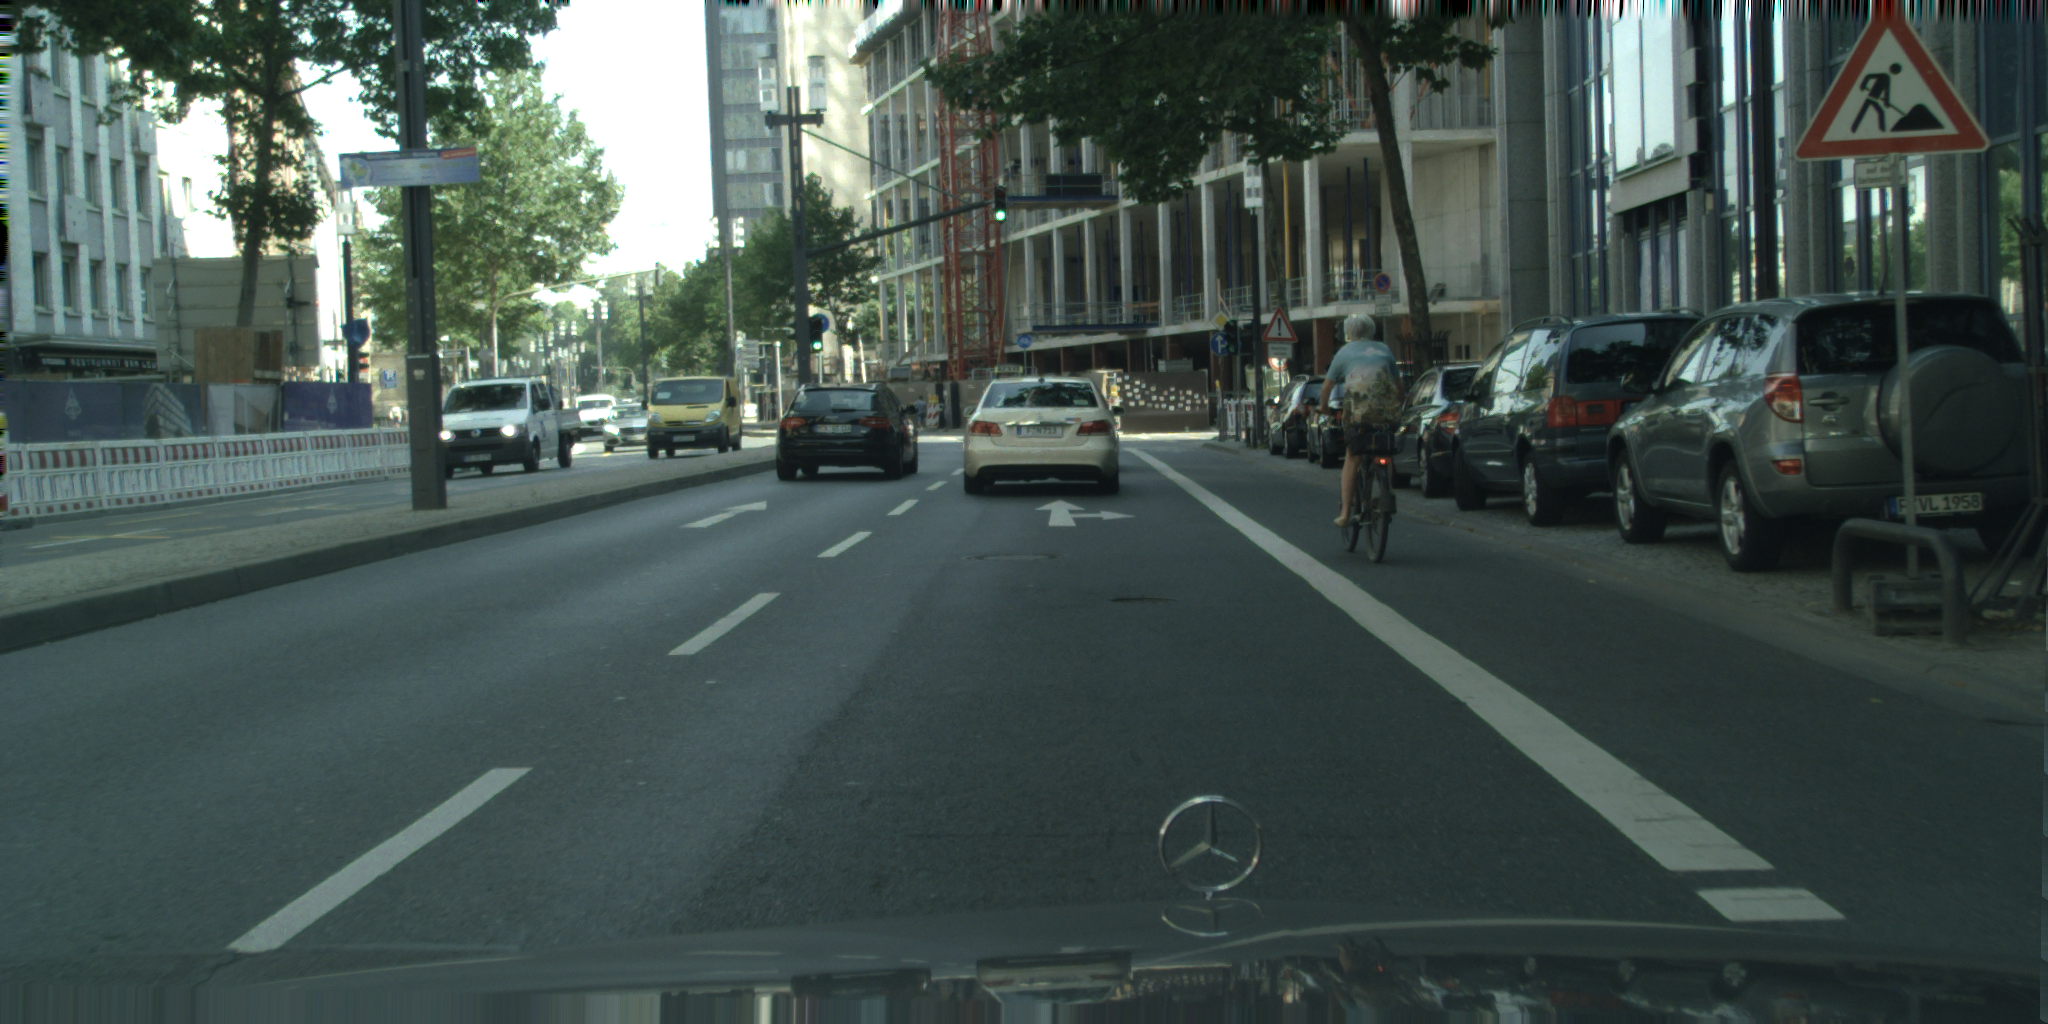
\includegraphics[width=0.67\linewidth]{Images/Original_frankfurt_000000_015676_leftImg8bit}
  \caption{\textgreek{Εικόνα εισόδου}}
  \end{subfigure}
 
 \begin{subfigure}[b]{\linewidth}
  \centering
  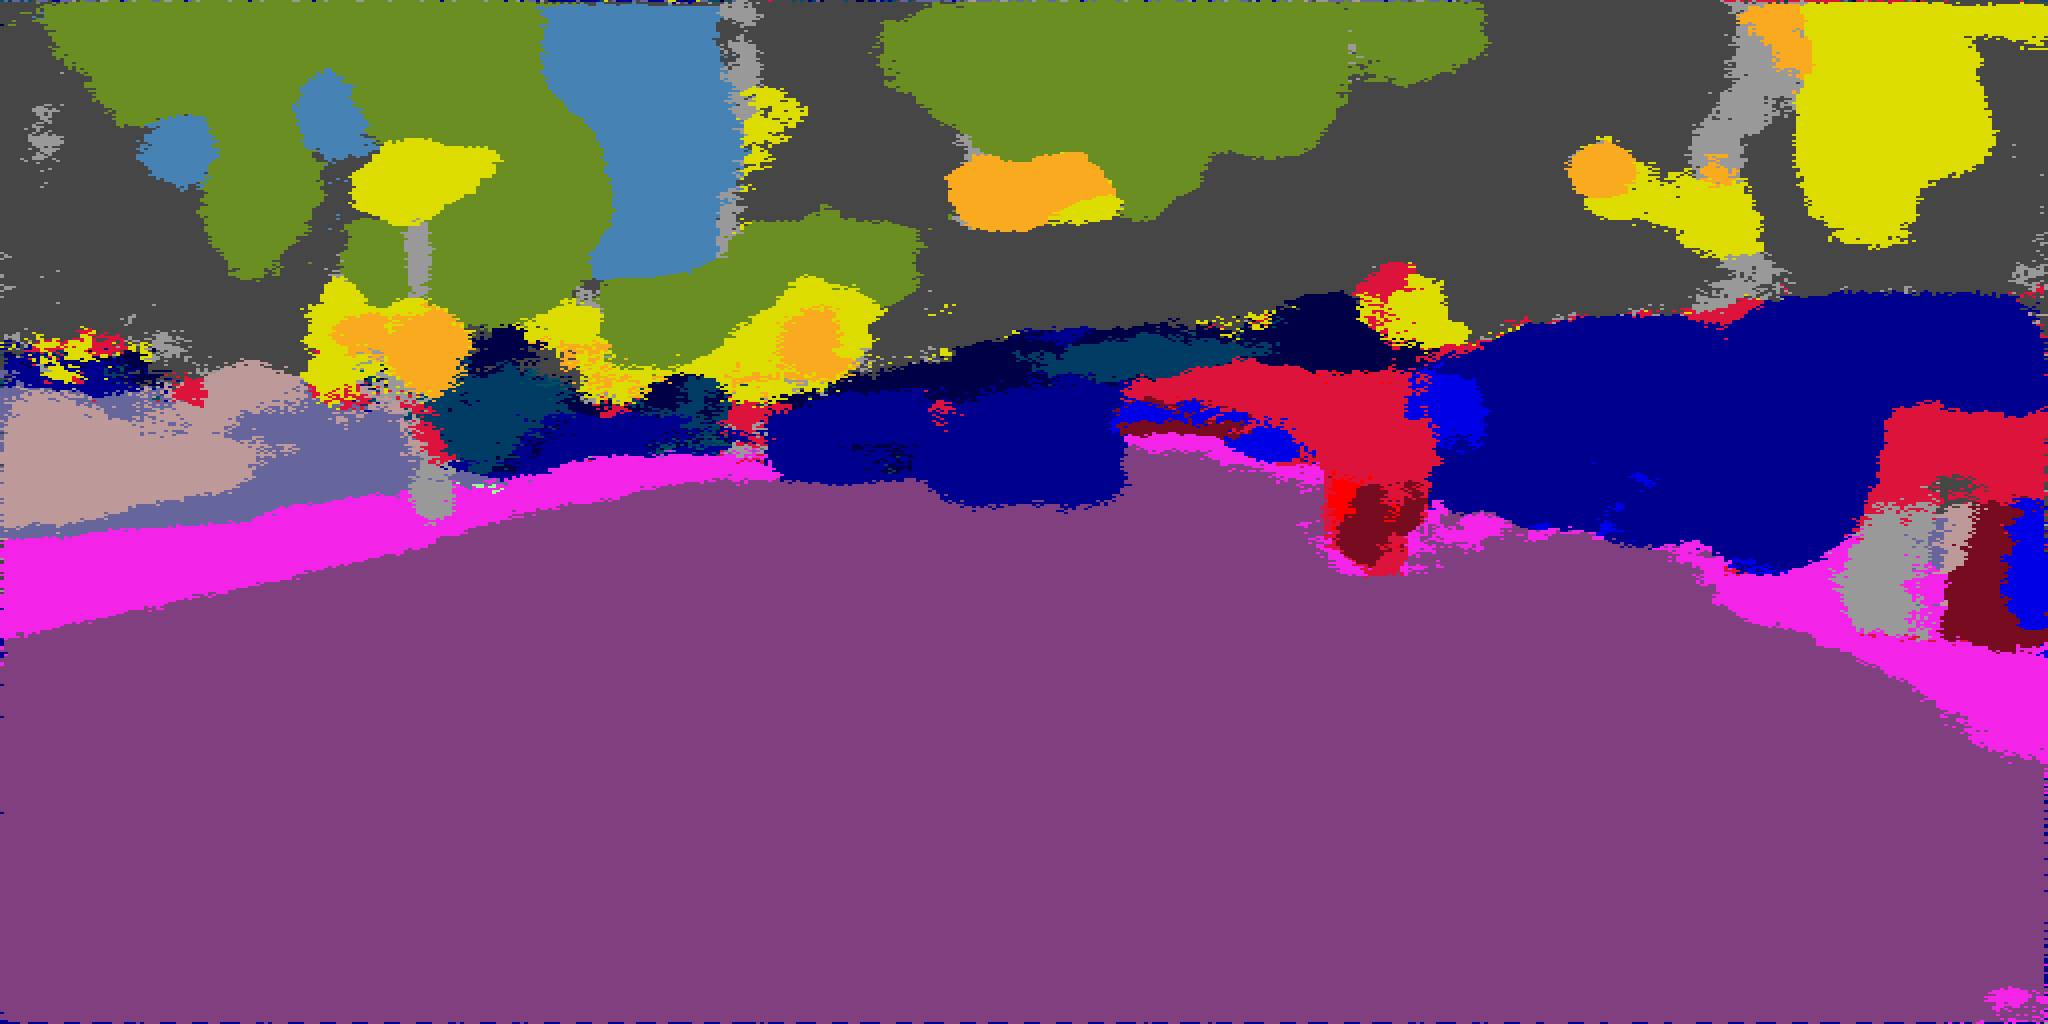
\includegraphics[width=0.67\linewidth]{Images/frankfurt_000000_015676_leftImg8bit_7_10_1024}
  \caption{\textgreek{Πρόβλεψη μοντέλου }SD-CNN-CRF-RNN.}
 \end{subfigure}
  
 \begin{subfigure}[b]{\linewidth}
  \centering
  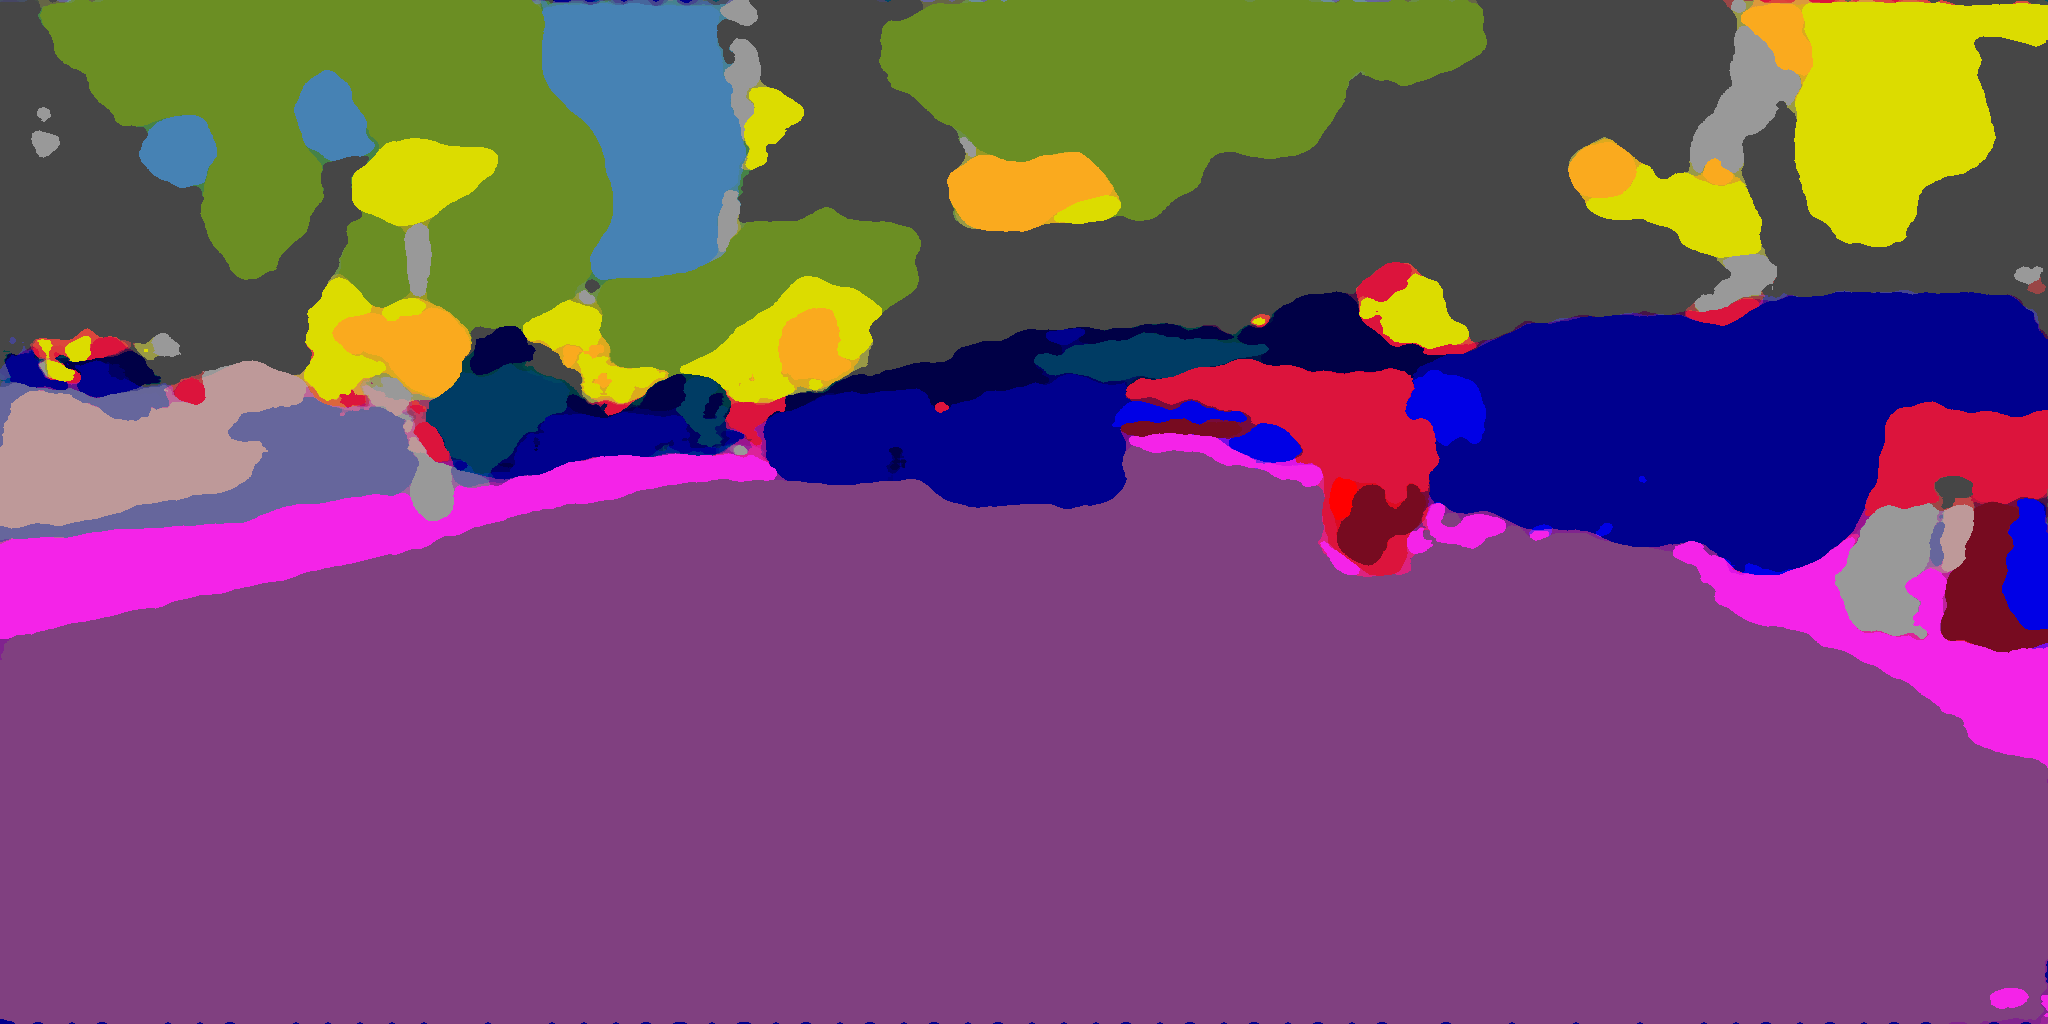
\includegraphics[width=0.67\linewidth]{Images/frankfurt_000000_015676_leftImg8bit_median_7_10_1024}
  \caption{\textgreek{Πρόβλεψη μοντέλου }SD-CNN-CRF-RNN \textgreek{με μεσαίο φίλτρο}.}
 \end{subfigure}
  
 \begin{subfigure}[b]{\linewidth}
  \centering
  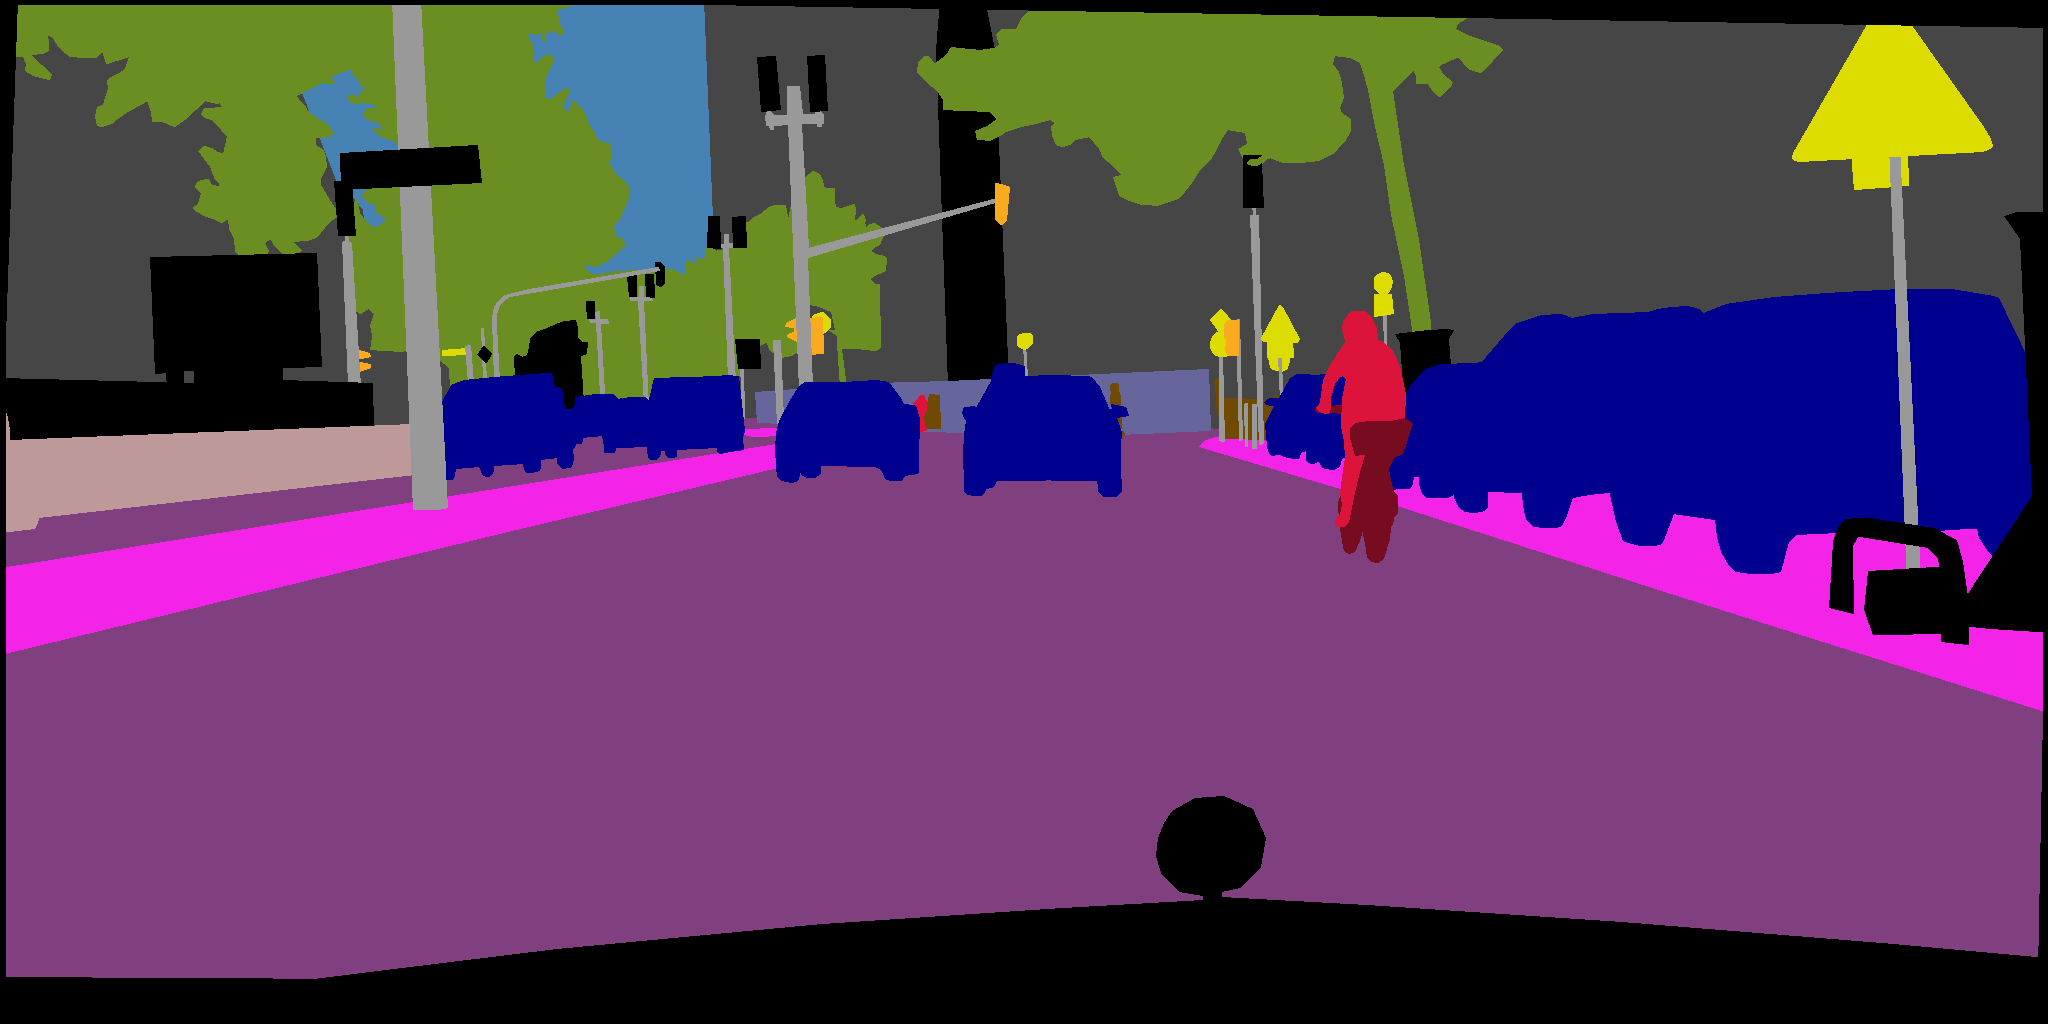
\includegraphics[width=0.67\linewidth]{Images/frankfurt_000000_015676_gtFine_color}
  \caption{Ground Truth}
 \end{subfigure}
  
  \caption[\textgreek{Εικόνες από ΠΣΝΔ-ΤΥΣΠ-ΕΝΔ}]{\textgreek{Εικόνες αποτελεσμάτων του ΠΣΝΔ με ΤΥΣΠ-ΕΝΔ με ισοστάθμιση κλάσεων.}}
 \label{fig:image_results_1}
\end{figure}

\begin{figure}[H]
 \centering
 \begin{subfigure}[b]{\linewidth}
 \centering
 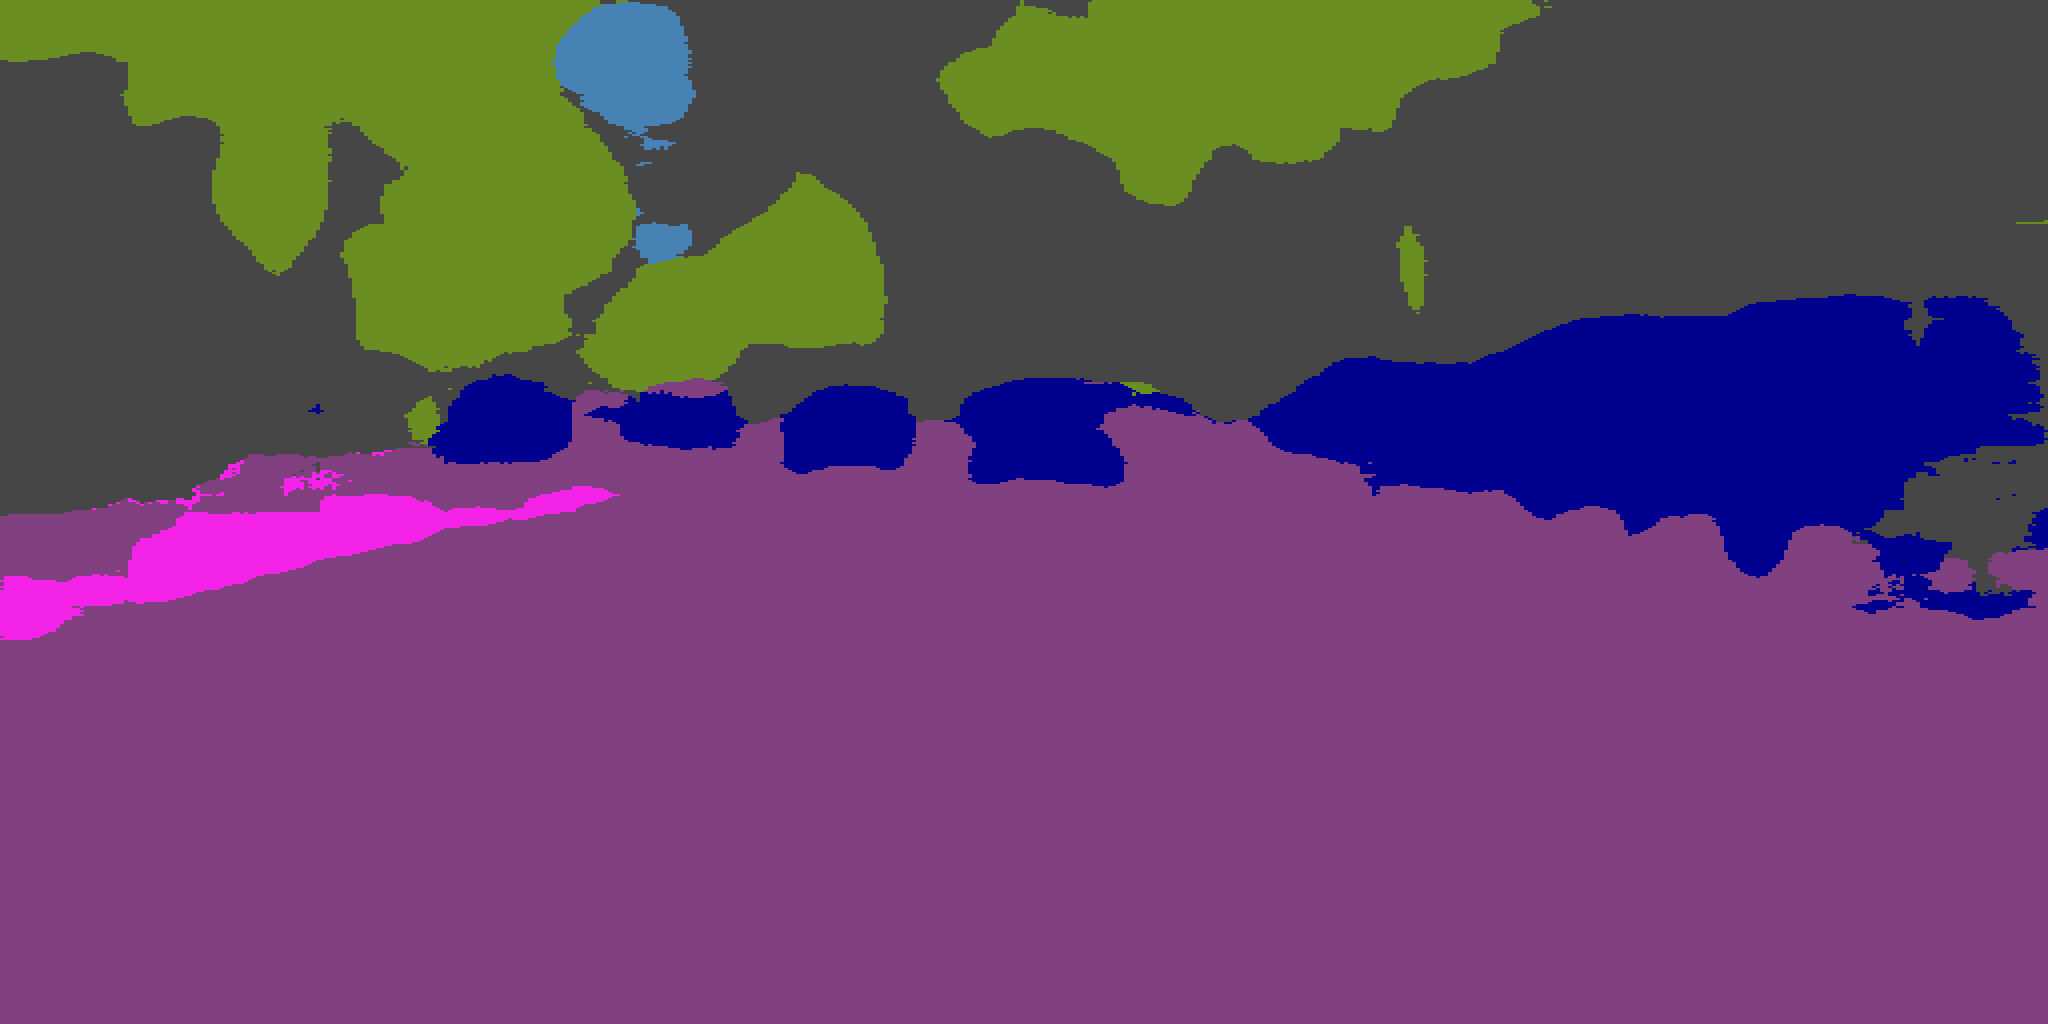
\includegraphics[width=0.8\linewidth]{Images/frankfurt_000000_015676_5_leftImg8bit}
  \caption{\textgreek{Πρόβλεψη μοντέλου }SD-CNN \textgreek{χωρίς ισοστάθμιση κλάσεων}.}
  \end{subfigure}
 ~
 \begin{subfigure}[b]{\linewidth}
 \centering
 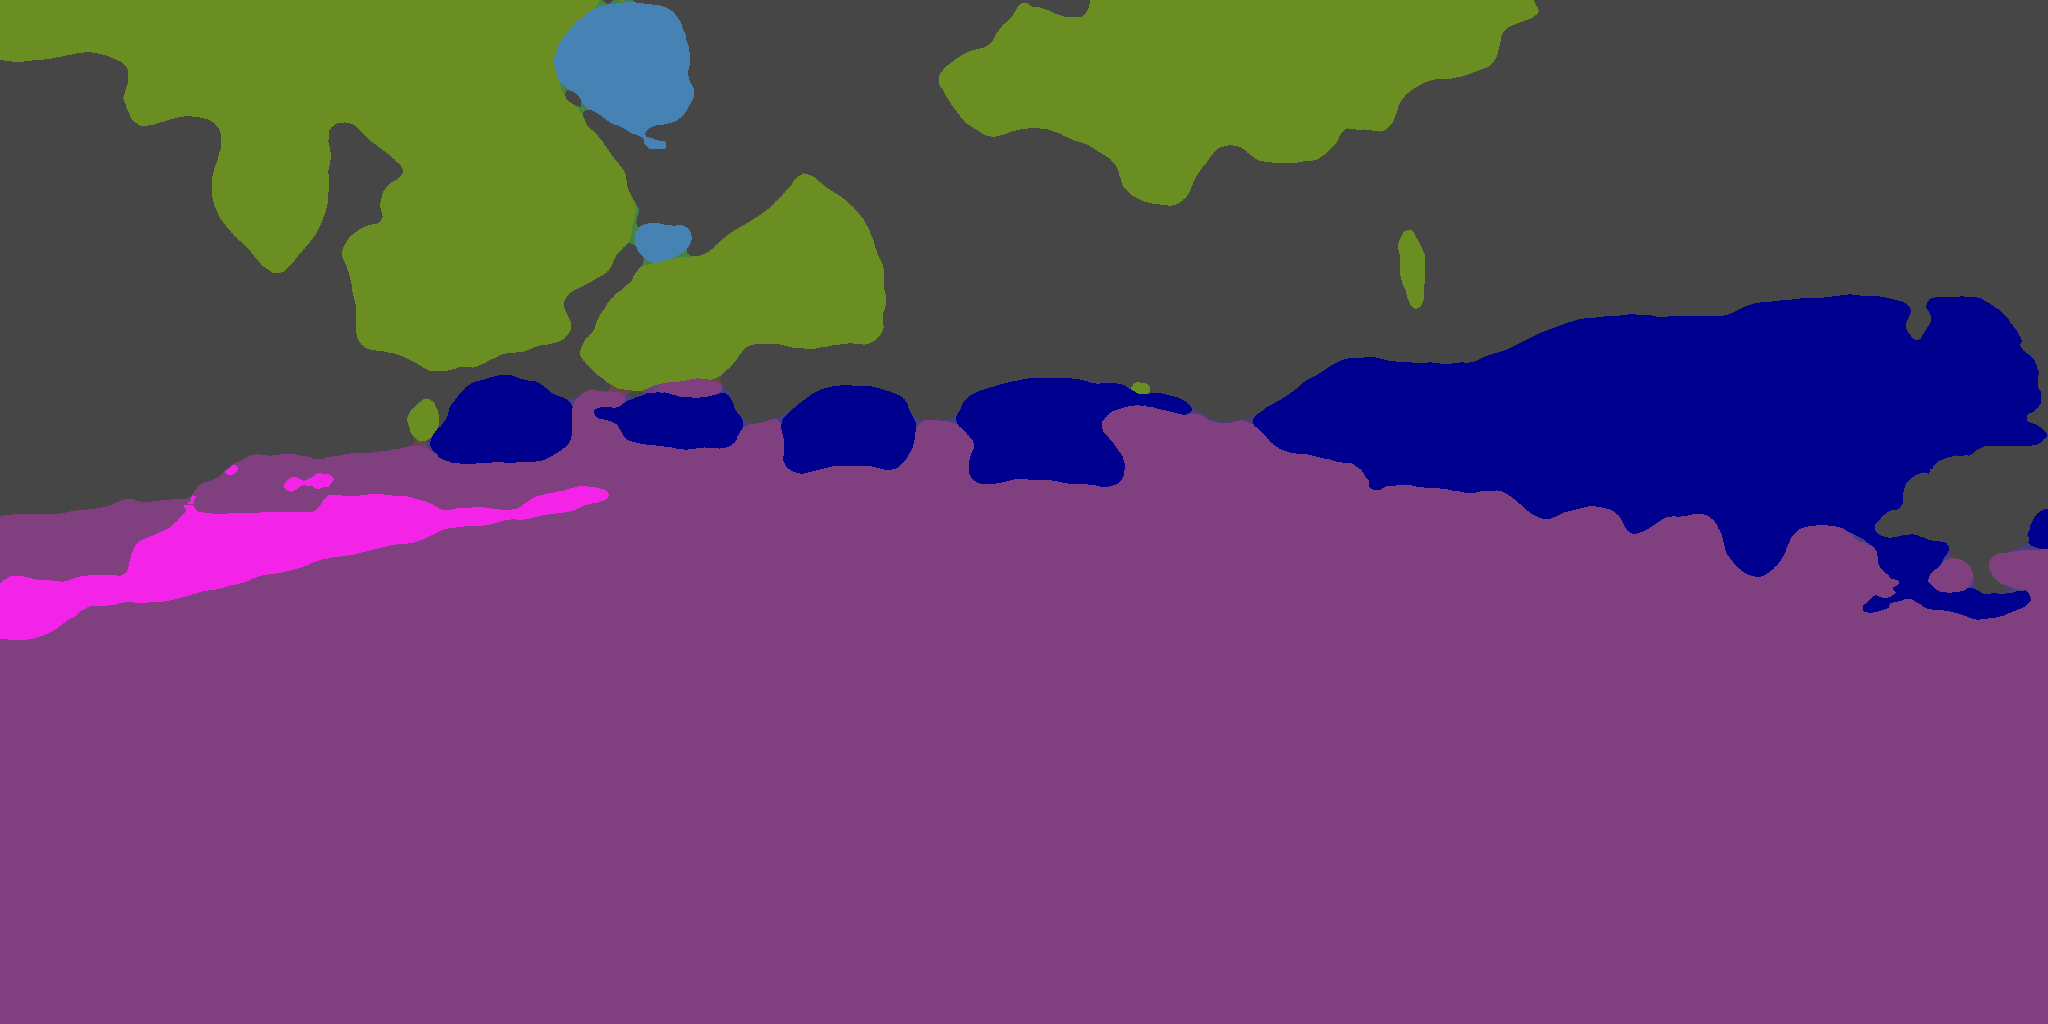
\includegraphics[width=0.8\linewidth]{Images/frankfurt_000000_015676_5_median_leftImg8bit}
  \caption{\textgreek{Πρόβλεψη μοντέλου }SD-CNN \textgreek{χωρίς ισοστάθμιση κλάσεων με την εφαρμογή του βέλτιστου παραθύρου μεσαίου φίλτρου}.}
  \end{subfigure}
  ~
  \begin{subfigure}[b]{\linewidth}
  \centering
  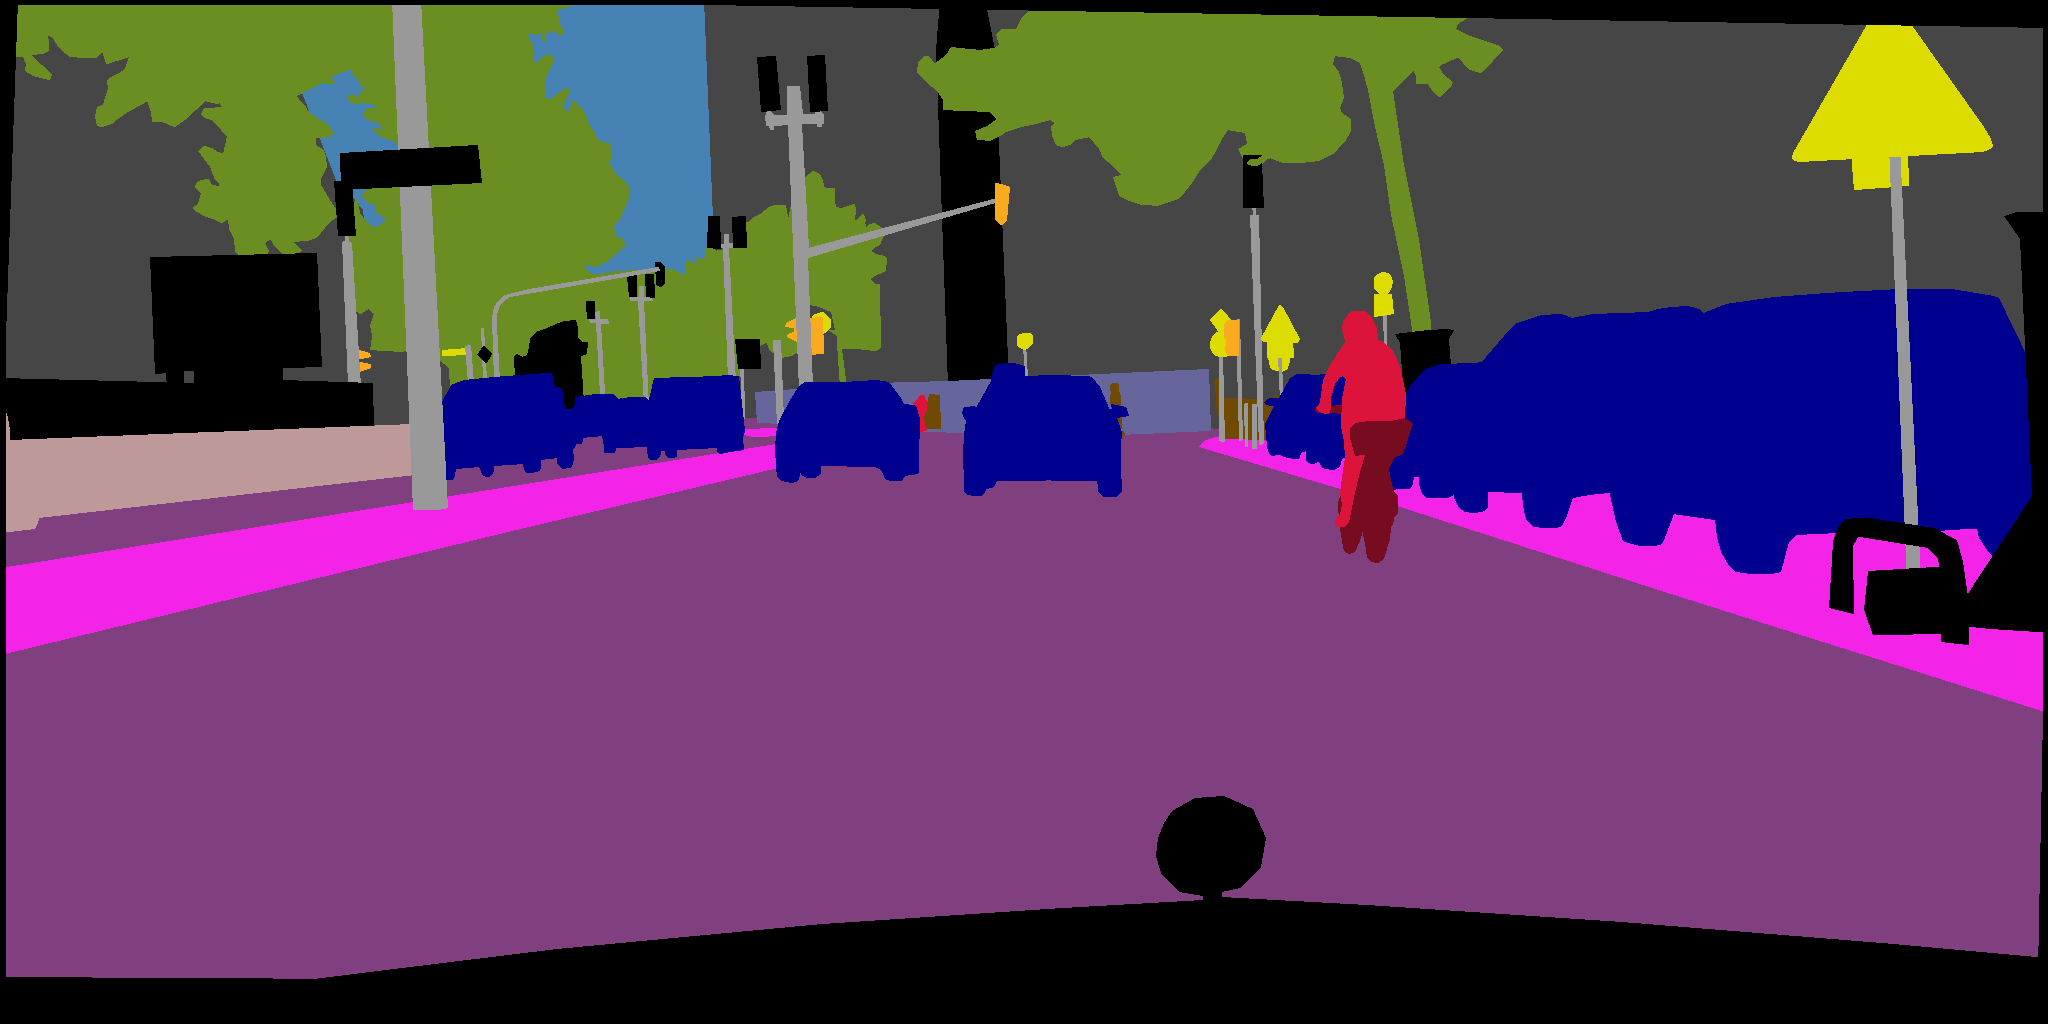
\includegraphics[width=0.8\linewidth]{Images/frankfurt_000000_015676_gtFine_color}
  \caption{Ground Truth}
 \end{subfigure}
  \caption[\textgreek{Εικόνες από ΠΣΝΔ}]{\textgreek{Εικόνες αποτελεσμάτων του ΠΣΝΔ χωρίς ισοστάθμιση κλάσεων με εφαρμογή μεσαίου φίλτρου και χωρίς.}}
 \label{fig:image_results_2}
\end{figure}

%%%%
\begin{figure}[H]
 \centering
 \begin{subfigure}[b]{\linewidth}
 \centering
 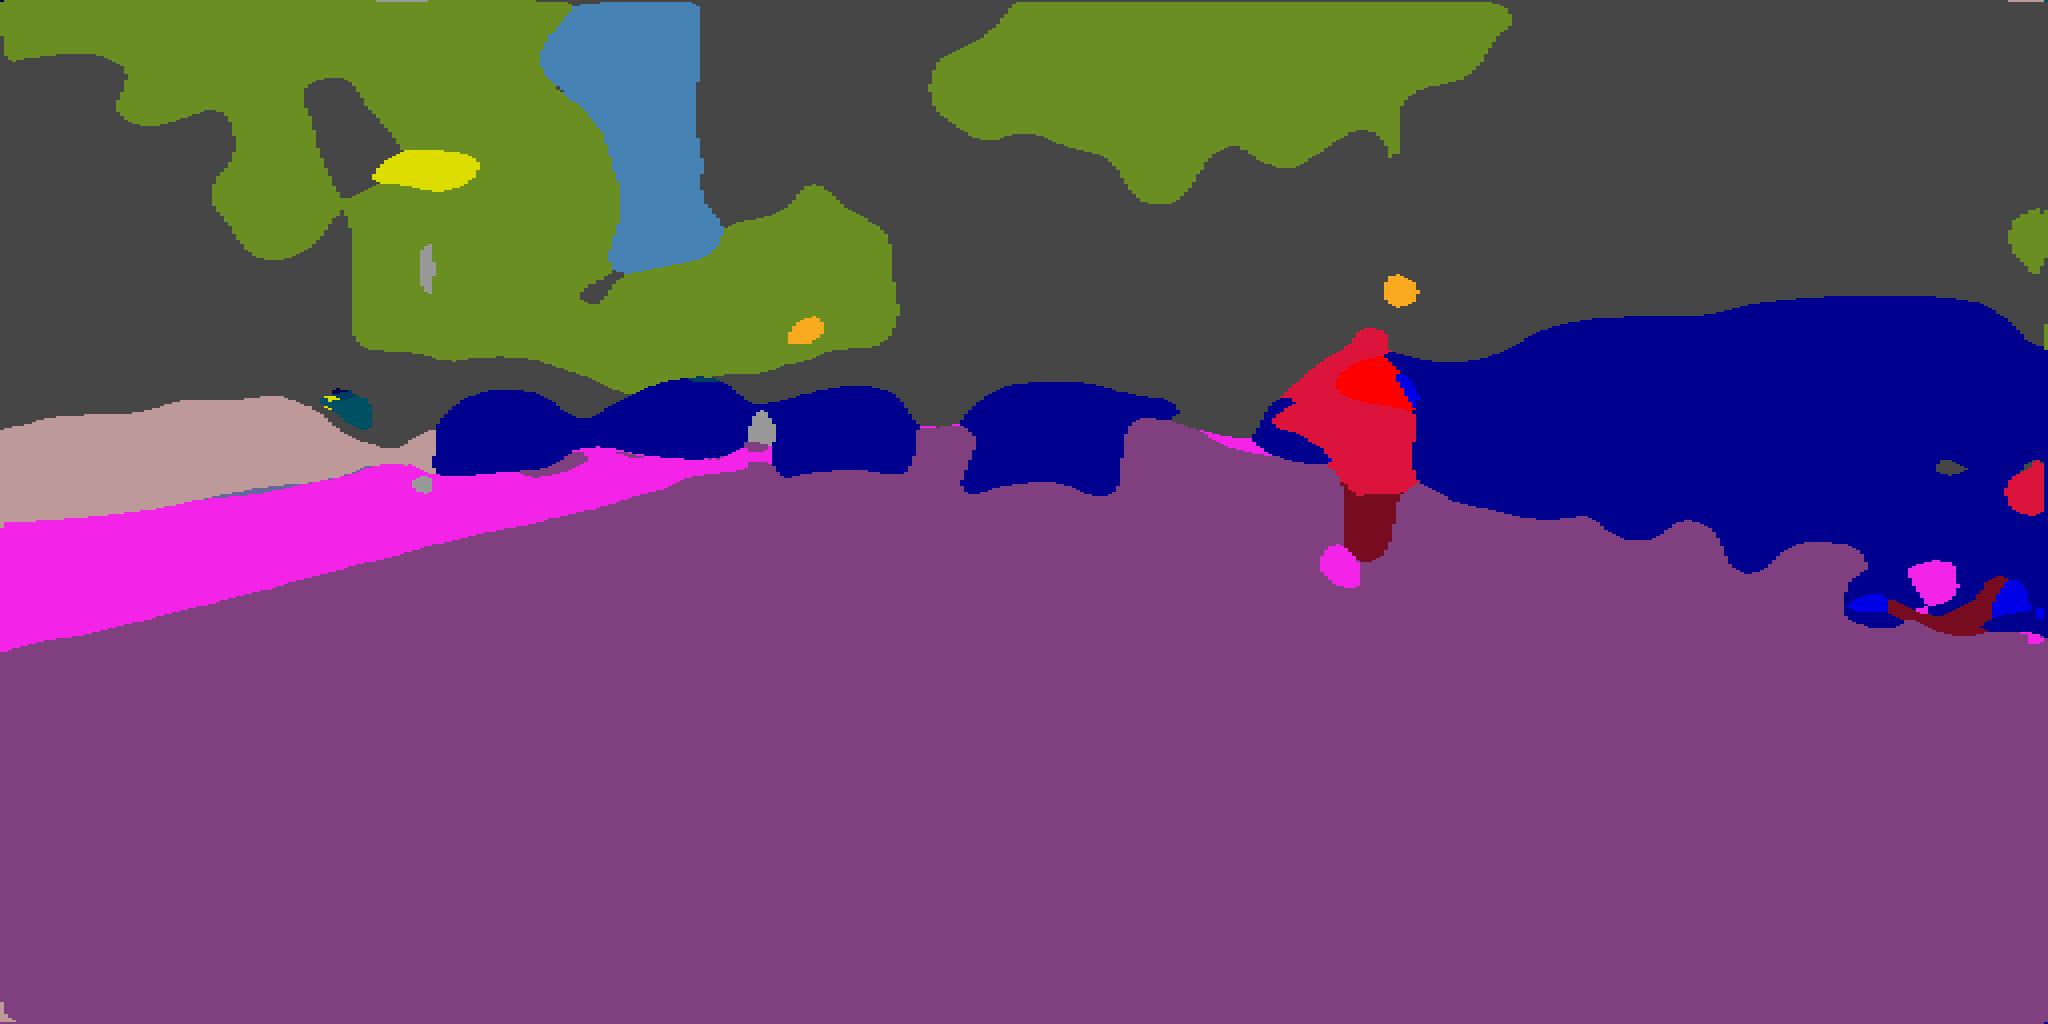
\includegraphics[width=0.8\linewidth]{Images/image_predictions_HighREs_512_11}
  \caption{\textgreek{Πρόβλεψη μοντέλου }BD-CNN \textgreek{χωρίς εφαρμογή φίλτρου}.}
  \end{subfigure}
 ~
 \begin{subfigure}[b]{\linewidth}
 \centering
 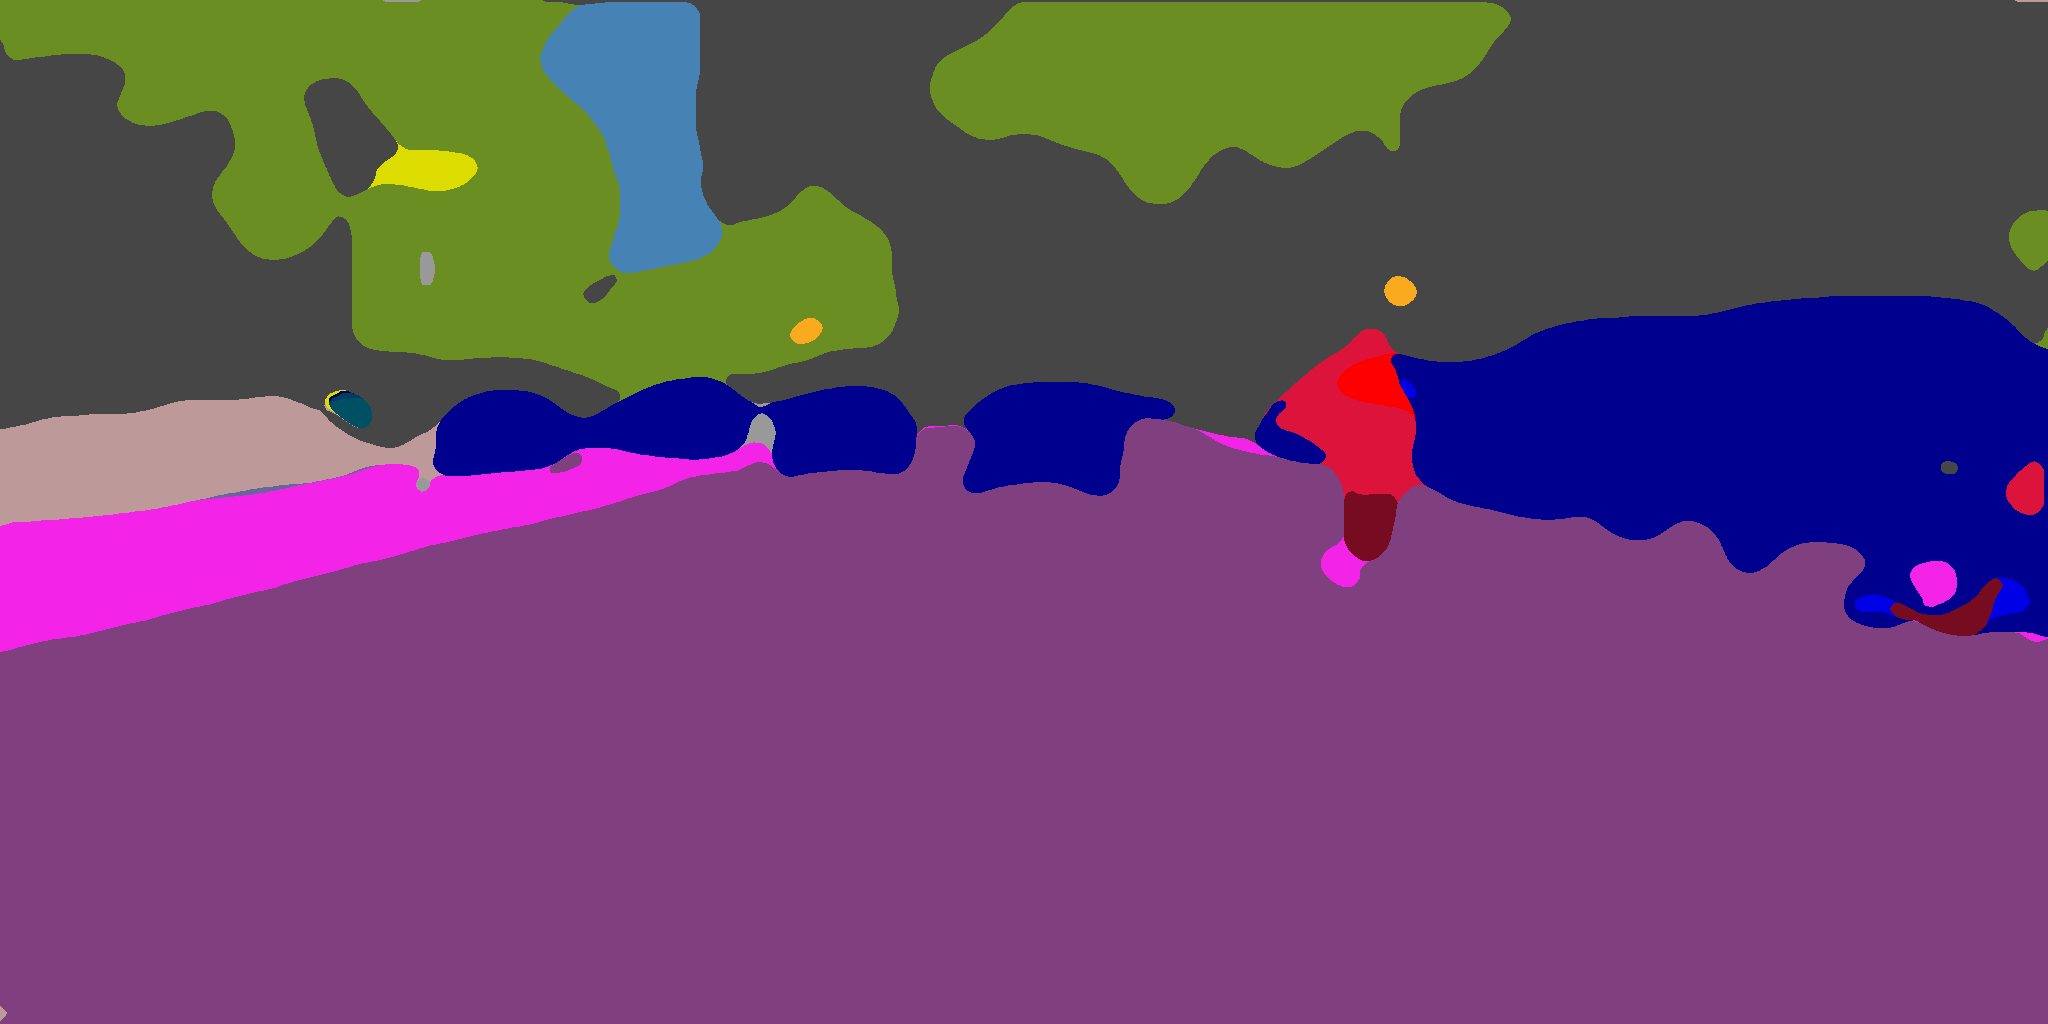
\includegraphics[width=0.8\linewidth]{Images/image_predictions_HighREs_median_512_11}
  \caption{\textgreek{Πρόβλεψη μοντέλου }BD-CNN \textgreek{με την εφαρμογή του βέλτιστου παραθύρου ($19\times 19$) του μεσαίου φίλτρου}.}
  \end{subfigure}
  ~
  \begin{subfigure}[b]{\linewidth}
  \centering
  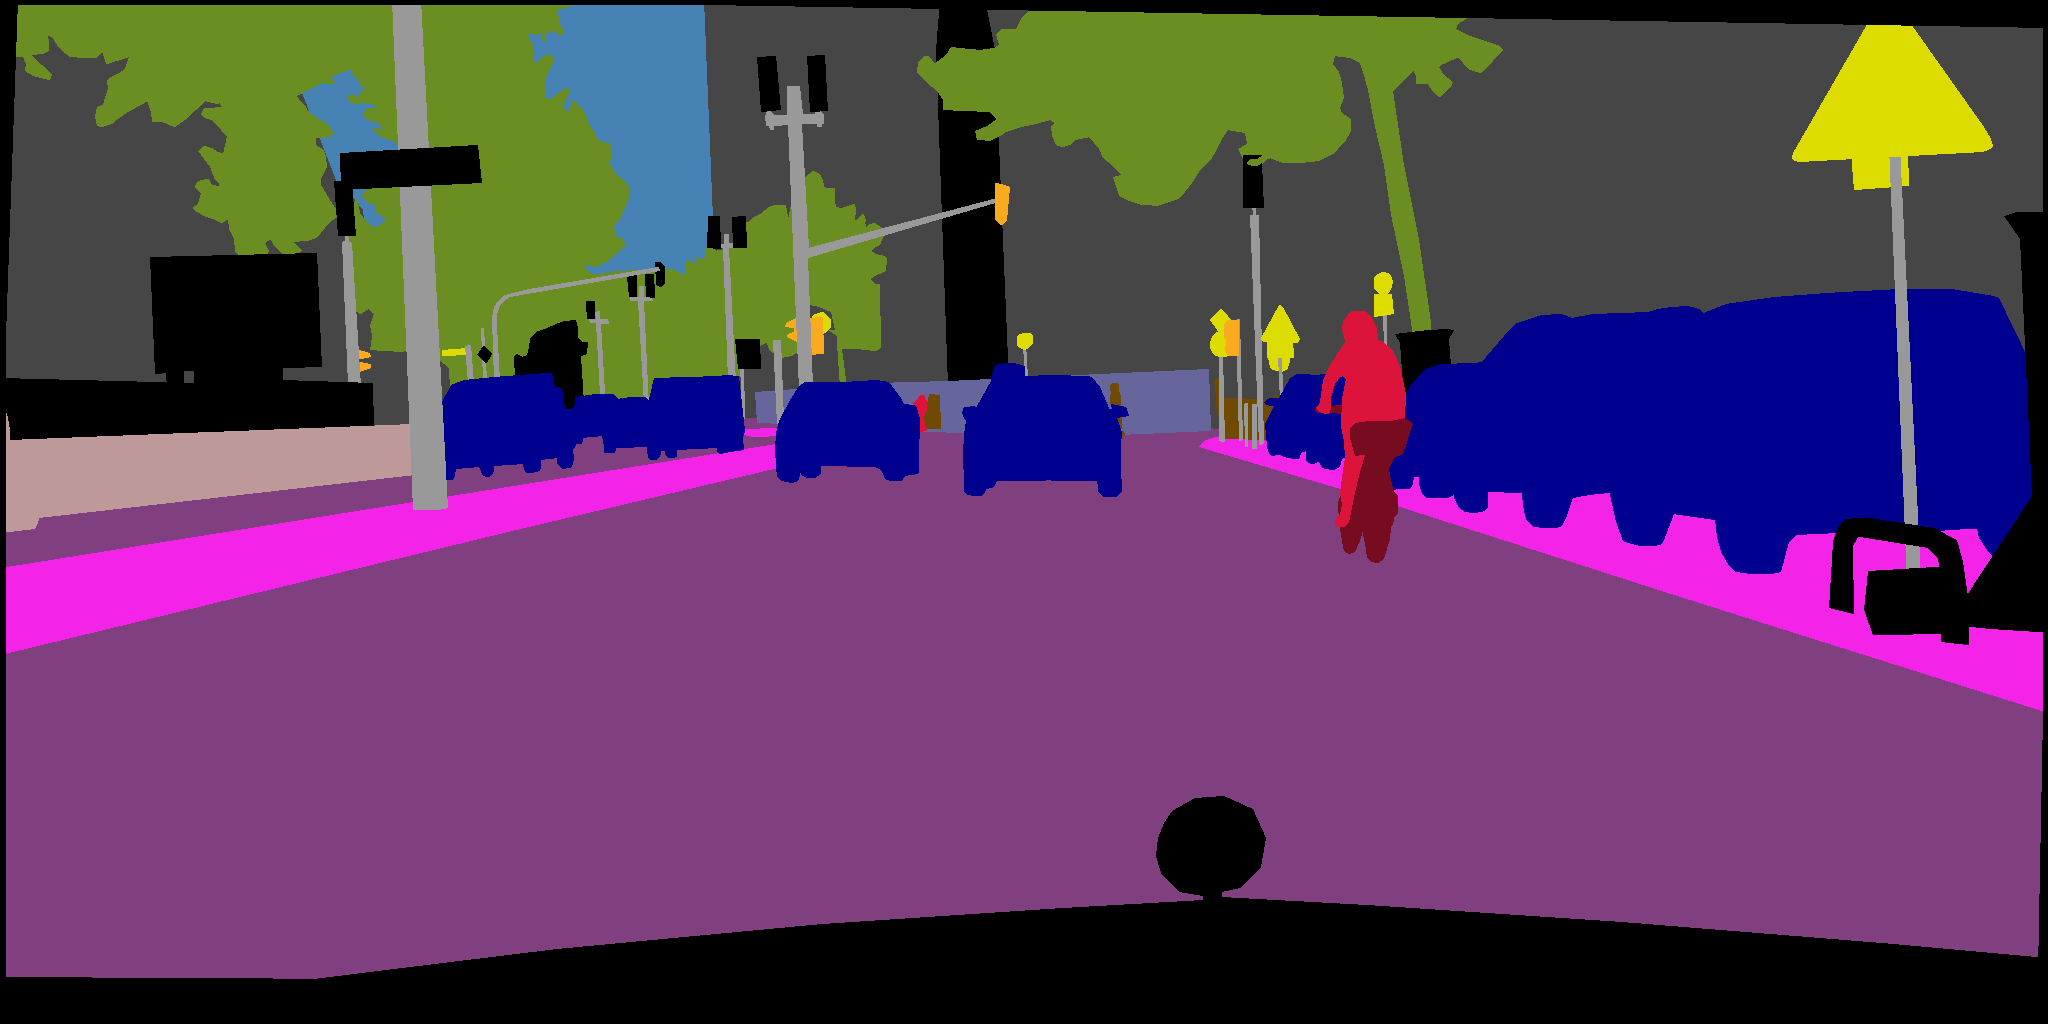
\includegraphics[width=0.8\linewidth]{Images/frankfurt_000000_015676_gtFine_color}
  \caption{Ground Truth}
 \end{subfigure}
  \caption[\textgreek{Εικόνες Διγραμμικών ΠΣΝΔ}]{\textgreek{Εικόνες αποτελεσμάτων του ΠΣΝΔ χωρίς ισοστάθμιση κλάσεων με εφαρμογή μεσαίου φίλτρου και χωρίς.}}
 \label{fig:image_results_3}
\end{figure}

\pagebreak
\textgreek{Οι πίνακες σύγχυσης που βλέπουμε παρακάτω στις εικόνες αποτελούν μια πιο αξιόπιστη μέθοδο οπτικοποίησης των αποτελεσμάτων για να δούμε πόσο ισχυρά είναι τα μοντέλα μας και ποιες κατηγορίες μπερδεύονται περισσότερο μεταξύ τους. Οι πίνακες παρουσιάζονται με μια κανονικοποιημένη μορφή, ενώ όσο πιο έντονο είναι το χρώμα στην διαγώνιο του πίνακα τόσο πιο δυνατό είναι το μοντέλο. Η μετρική }Jaccard Similarity \textgreek{που είδαμε προηγουμένως επειδή υπολογίζει καθολικά σε όλη την εικόνα τις παραμέτρους της και βγάζει μια μέση τιμή από αυτές δεν δύναται να μας δώσει σωστά την ακρίβεια για κάθε κατηγορία. Στην αριστερή πλευρά των πινάκων σύγχυσης έχουμε τις πραγματικές κατηγοριοποιήσεις των εικονοστοιχείων ενώ κάθετα έχουμε τις προβλέψεις των μοντέλων μας. Η τελευταία στήλη και σειρά ανήκουν στην κατηγορία 'χωρίς ετικέτα' για αυτό και το αφήσαμε κενό. \par  }

\textgreek{Η εικόνα }\ref{fig:cf_1} \textgreek{μας συγκρίνει τα μοντέλα που δεν έχουν εκπαιδευτεί με την μέθοδο της ισοστάθμισης. Για τους λόγους που εξηγήσαμε προηγουμένως, το μοντέλο με την διγραμμική μονάδα (εικόνα }\ref{fig:image_results_3}) \textgreek{τα πηγαίνει αρκετά καλύτερα.}

\textgreek{Τέλος, στην εικόνα }\ref{fig:cf_2} \textgreek{επιδεικνύεται η σύγκριση μεταξύ του μοντέλου }SD-CNN \textgreek{με ισοστάθμιση των κλάσεων (εικόνα} \ref{fig:image_results_2}) \textgreek{καθώς και του }end-to-end \textgreek{μοντέλου }SD-CNN-CRF-RNN \textgreek{ με αριθμό επαναλήψεων επανεκτίμησης ίσο με πέντε. Η διαφορά μεταξύ των δύο μοντέλων δεν είναι πολύ μεγάλη άλλωστε όπως είδαμε και πριν ήταν μόλις 1\%. Όμως μπορούμε να δούμε πως πολλές λανθασμένες προβλέψεις έχουν μειωθεί αρκετά και αυτό δείχνει την ισχύ του μοντέλου μετα-επεξεργασίας. Αξίζει να δούμε την κλάση μοτοσυκλέτα η οποία έχει μειωθεί στο ΤΥΣΠ-ΕΝΔ. Πιθανόν τα εικονοστοιχεία που ταιριάζουν σε αυτή την κλάση, μοιάζουν αρκετά με εικονοστοιχεία κάποιας άλλης κλάσης και για αυτό τυχαίνει να υπάρχει μείωση. Οι πίνακες σύγχυσης υπολογίστηκαν πάνω στις 500 εικόνες του συνόλου δεδομένων επαλήθευσης στο αρχικό μέγεθος της εικόνας.} 

%%%% CONFUSION MATRICES
\newpage
\begin{figure}[H]
\centering
\begin{subfigure}[b]{\linewidth}
 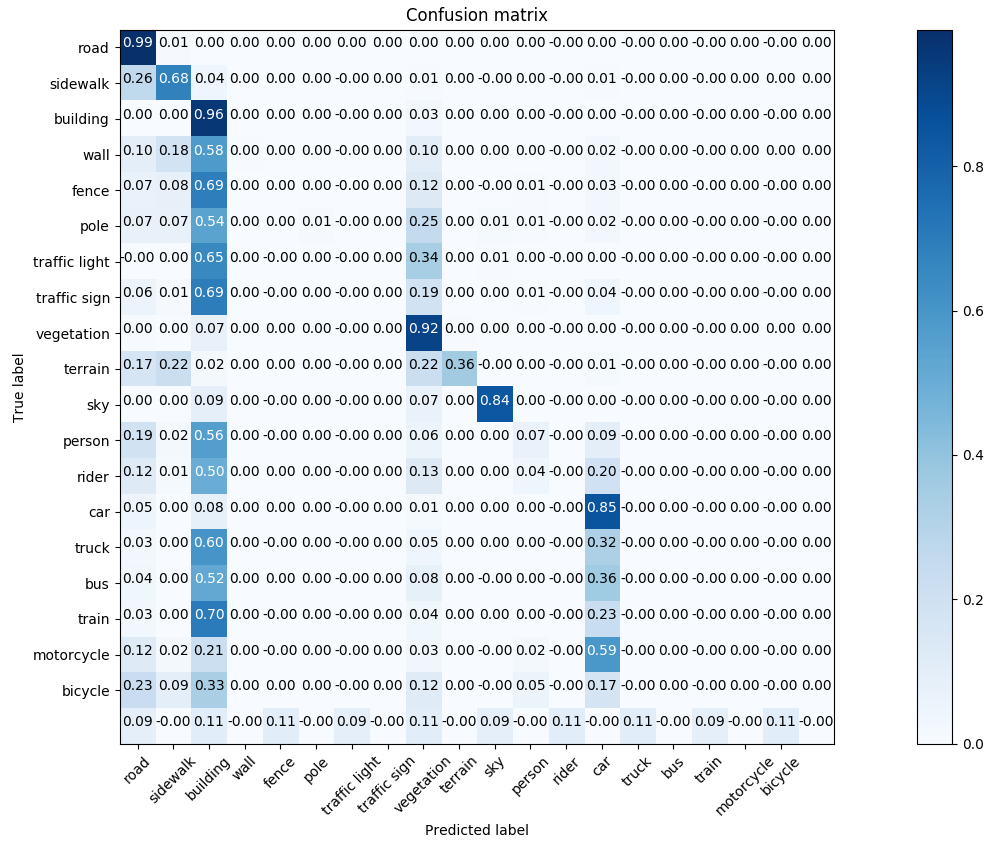
\includegraphics[scale=0.38 ]{Images/final_CF_5}
 \caption{\textgreek{Πίνακας Σύγχυσης του ΠΣΝΔ με μονάδα αποκωδικοποίησης με άλμα ολίσθησης} (SD-CNN)\textgreek{ χωρίς εφαρμογή της συνάρτησης ισοστάθμισης.}}
\end{subfigure}
\\[1pt]
\begin{subfigure}[b]{\linewidth}
 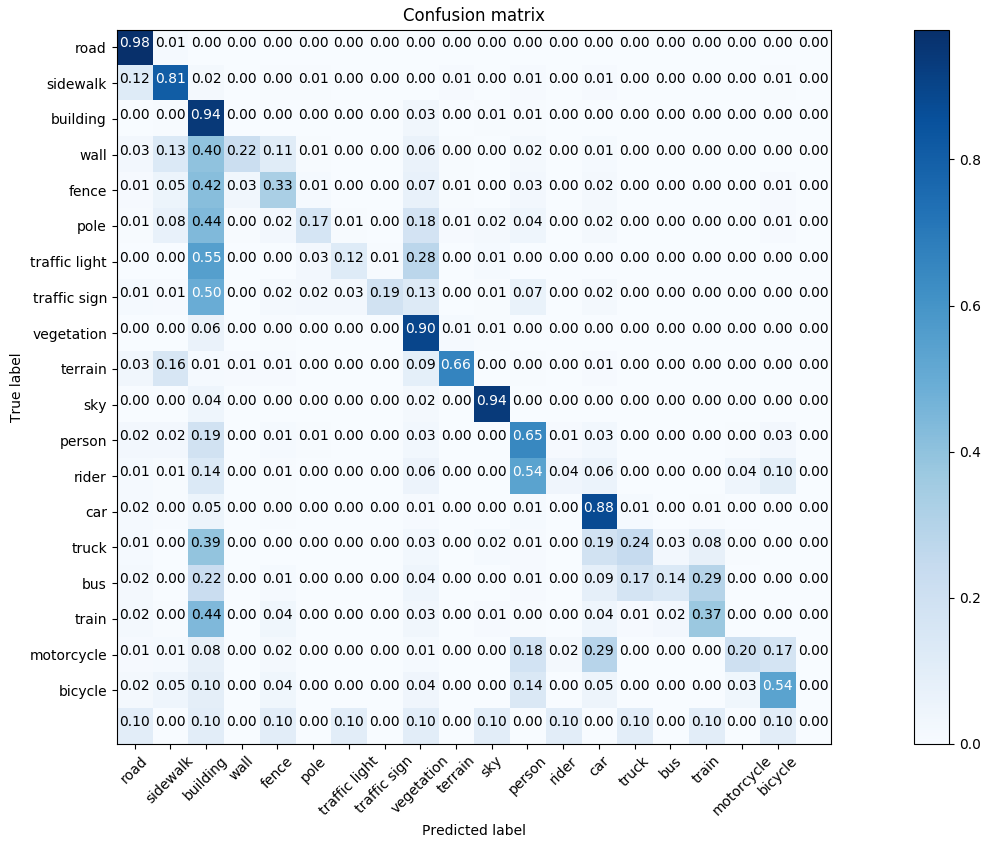
\includegraphics[scale=0.38]{Images/final_CF_11}
 \caption{\textgreek{Πίνακας Σύγχυσης του ΠΣΝΔ με διγραμμική μονάδα αποκωδικοποίησης} (BD-CNN)\textgreek{ χωρίς εφαρμογή της συνάρτησης ισοστάθμισης.}}
 \end{subfigure}
 
\caption[\textgreek{Πίνακες Σύγχυσης χωρίς μετα-επεξεργασία}]{\textgreek{Πίνακες σύγχυσης των μοντέλων χωρίς μονάδες μετα-επεξεργασίας και ισοστάθμιση των κλάσεων.}}
\label{fig:cf_1}
\end{figure}


\begin{figure}[H]
\centering
\begin{subfigure}[b]{1\linewidth}
 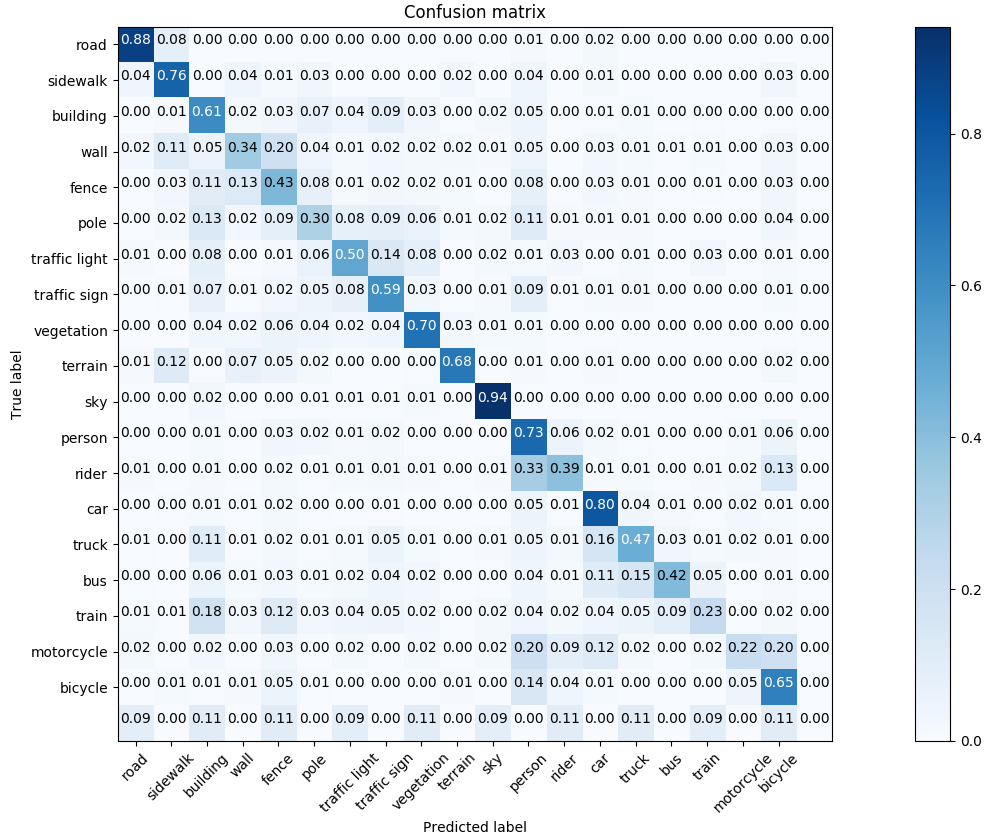
\includegraphics[scale=0.36]{Images/final_CF_7} \\[1pt]
 \caption{\textgreek{Πίνακας Σύγχυσης του ΠΣΝΔ με μονάδα αποκωδικοποίησης με άλμα ολίσθησης} (SD-CNN)\textgreek{ με ισοστάθμιση των κλάσεων.}}
 \end{subfigure}
\begin{subfigure}[b]{1\linewidth}
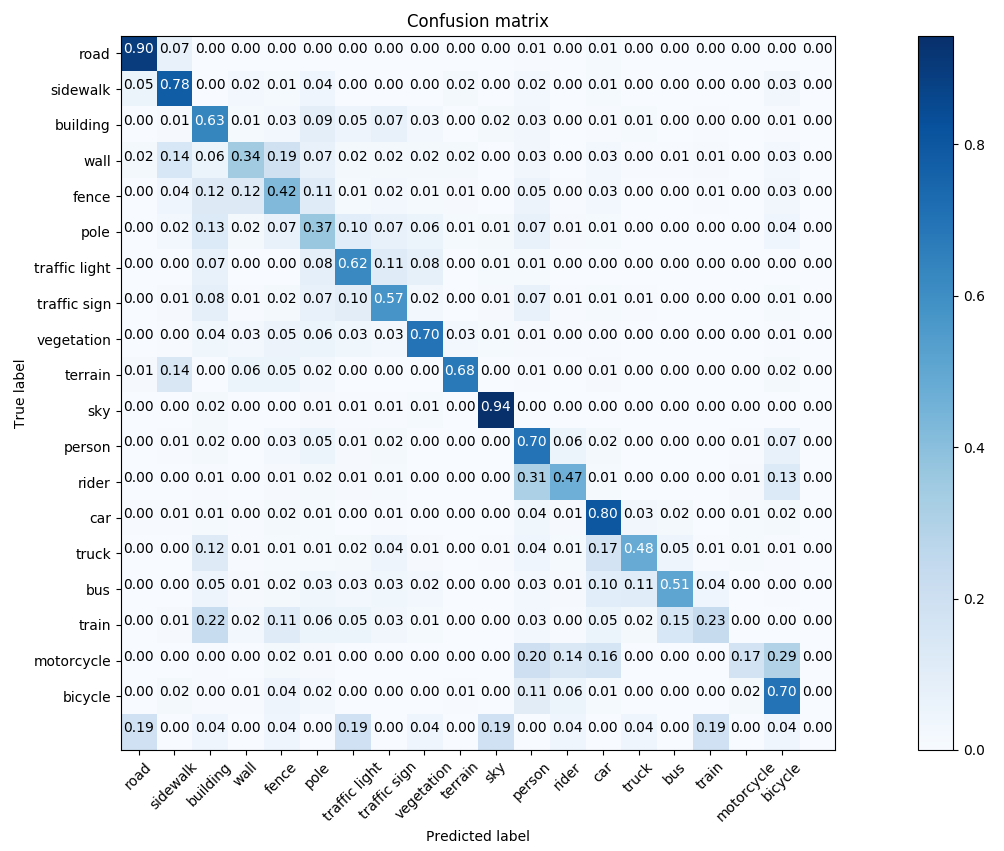
\includegraphics[scale=0.36]{Images/final_CF_7_CRF5}
\caption{\textgreek{Πίνακας Σύγχυσης του ΠΣΝΔ με μονάδα αποκωδικοποίησης με άλμα ολίσθησης και με μονάδα μετα-επεξεργασίας ΤΥΣΠ-ΕΝΔ} (SD-CNN-CRF)\textgreek{ με ισοστάθμιση των κλάσεων.}}
\end{subfigure}
\caption[\textgreek{Πίνακες Σύγχυσης με ΤΥΣΠ-ΕΝΔ}]{\textgreek{Πίνακες σύγχυσης για την σύγκριση των μοντέλων με και χωρίς μονάδα μετα-επεξεργασίας και ισοστάθμιση των κλάσεων.}}\label{fig:cf_2}
\end{figure}
